% Chapter Template

\chapter{Theoretical overview and previous measurements} % Main chapter title

\label{Chapter2} 

\lhead{Chapter 2. \emph{Theoretical overview}} % Change X to a consecutive number; this is for the header on each page - perhaps a shortened title

The standard model of elementary particles is a theory which emerged in the 1960s and 1970s, describing all of the known elementary particles and interactions except gravity. The final formulation of the Standard model incorporates several theories: quantum electrodynamics, Glashow-Weinberg-Salam theory of electroweak processes and quantum chromodynamics. The first steps towards formulation of Standard model occurred in 1961. when Sheldon Glashow unified electromagnetic and weak interactions\cite{Glashow1961579}. The difference in strength between the weak and electromagnetic forces was puzzling for physicists at that time, and Glashow proposed that it can be accounted for if the weak force were mediated by massive bosons. However, he was not able to explain the origin of the mass for such mediators. The explanation came in 1967. when Steven Weinberg and Abdul Salam used the Higgs mechanism in the electroweak theory\cite{PhysRevLett.19.1264,Salam:1968rm}, which suggested the existence of an additional particle called Higgs boson. After the discovery of neutral currents, which arise from the exchange of the neutral Z boson, the electroweak theory became generally accepted. The W and Z bosons were discovered in 1983 at CERN\cite{Arnison1983103,Arnison1983398}, and their masses were in agreement with the standard model prediction. The theory describing strong interactions got its final form in 1974. when it was shown that hadrons consist of quarks. The final missing link in the Standard model, the Higgs boson, was discovered in 2012 at CERN\cite{Aad:2012tfa,Chatrchyan:2012ufa}. There are several unexplained phenomena which suggest the existence of physics beyond Standard model, but so far its predictions were confirmed every time through numerous experimental tests.  \\
In this chapter a brief overview of the Standard model particles and interactions will be shown with the emphasis on the W boson and b quarks, which are the most relevant for this thesis. An introduction to cross section determination at hadron colliders is given. In the last part of the chapter an historical overview of the development of W+b-jets theoretical calculations is described together with the existing experimental results.

%----------------------------------------------------------------------------------------
%	SECTION 1
%----------------------------------------------------------------------------------------

\section{Standard model overview}

\par Elementary particle physics is described within the framework of the Standard model. We usually imagine particles as point like objects and some forces between them. These particles are fermions, leptons or quarks of spin $s=1/2$. There are three charged leptons, electron, muon and tau whose properties are the same except for their mass. Each of the leptons has a corresponding neutrally charged neutrino with a very small mass. There are six different types of quarks with charge either $Q=2/3$ of $Q=-1/3$. They also carry one additional quantum number, which is color charge. All objects observed in nature are colorless giving rise to the concept of quark confinement, which will be explained later. Colorless composite objects are classified into two categories. Bayons are fermions made out of three  quarks, for example proton or neutron. The other category is composed of mesons, which are made of quark and antiquark, like pions. Quarks are divided into three generations with all identical properties except for the masses of the particles. 
\par The standard model is based on a gauge symmetry $SU(3)_C \times SU(2)_L \times U(1)_Y$. Strong interaction symmetries are described by $SU(3)_C$ group, while the electroweak sector is described by $SU(2)_L \times U(1)_Y$. All interactions within the standard model are mediated by elementary particles which are a spin 1 bosons. In the case of electromagnetic interactions, the mediator is a massless photon. Thus the range of electromagnetic interaction is infinite. For the weak force the mediators are the three massive bosons $W^{\pm}$ and $Z$ and its range is very small ($10^{-16}$ m). These four bosons are the gauge bosons of the $SU(2)_L \times U(1)_Y$ group. The interaction between electroweak bosons is allowed in the standard model as long as charge conservation principle remains valid. The strong force is mediated by the exchange of 8 massless gauge bosons for $SU(3)_C$ called gluons. Although gluons are massless, the range of the strong force is not infinite. Due to the effect of confinement, the range of the strong force is approximately the size of the lightest hadrons ($10^{-13} cm$). 
\begin{figure}[htbp]
	\centering
		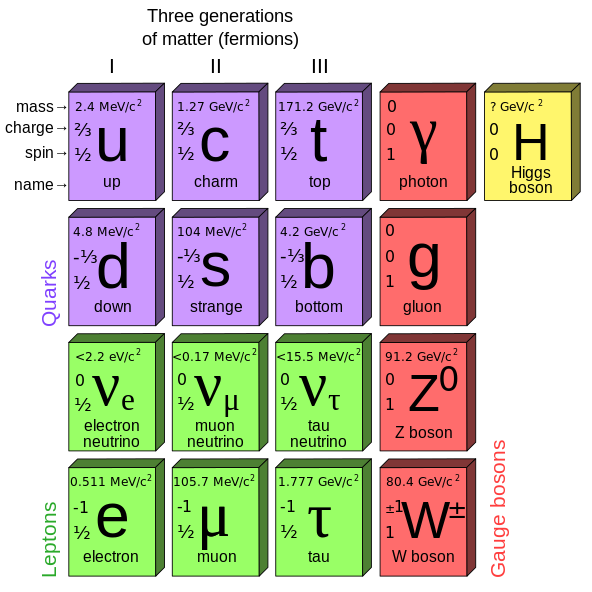
\includegraphics[width=0.5\textwidth]{Figures/Elementary_Particles.png}
		%\rule{35em}{0.5pt}
	\caption[List of Standard model elementary particles]{List of Standard model elementary particles.}
	\label{fig:SM_particles}
\end{figure} 
\par The fact that weak gauge bosons are massive indicates that $SU(2)_L \times U(1)_Y$ is not a good symmetry of the vacuum. Photons, on the other hand, are massless, $U(1)_{em}$ is thus a good symmetry of the vacuum. This means that the $SU(2)_L \times U(1)_Y$ electroweak symmetry is somehow spontaneously broken to $U(1)_{em}$ of electromagnetism. Spontaneous symmetry breaking is implemented through the Higgs mechanism, which gives masses to fermions, $W^{\pm}$ and $Z$ boson and leaves the photon massless. Details of the mechanism can be found elsewhere, e.g. \cite{Griffiths:1987tj} but the main point is that it also predicts a new scalar and electrically neutral particle which is called Higgs boson. The search for the Higgs boson lasted few decades before finally in 2012, a new particle was discovered with a mass of 125 GeV \cite{Aad:2012tfa,Chatrchyan:2012ufa}. In subsequent years, properties of this new particle have been measured. At this point, all measurements agree with Standard Model predictions for the Higgs boson.    
   

%-----------------------------------
%	SUBSECTION 1.1
%-----------------------------------

\subsection{Bottom quark}

The history of the bottom quark begins in 1973, when Makoto Kobayashi and Toshihide Maskawa first introduced the third generation of quarks to explain the CP violation observed in neutral K mesons \cite{Kobayashi:1973fv}. CP violation is introduced as a small phase factor $\delta$ in the Cabibbo-Kobayashi-Maskawa (CKM) matrix provided there are at least three generations of quarks. This prediction was done even before the discovery of c quark. Kobayashi and Maskawa winning the 2008 Nobel Prize in Physics for their explanation of CP-violation after several experiments confirmed that the predicted behavior is not exclusive for K mesons, but can be seen also in B mesons \cite{Aubert:2001sp,Abe:2001xe}.
\par The name "bottom" was introduced in 1975 by Haim Harari. The bottom quark was discovered in 1977 by the Fermilab E288 experiment team led by Leon M. Lederman through the observation of the $\Upsilon$ resonance, which is formed from a bottom quark and its antiparticle \cite{PhysRevLett.39.252}.  
\par At the LHC, the main production mechanism for b quarks is through strong interaction (any diagram involving $g\rightarrow bb$). Other important contribution for this analysis is also from top quark decay ($t\rightarrow Wb$). Every b quark, after production, goes through the process of hadronization, forming one of the color neutral B hadrons. Excited B hadrons decay strongly or electromagnetically, while ground state B hadrons decay weakly, resulting in relatively long lifetime of $\sim$1.5 ps. Bottom quark can decay either to c quark or u quark. Both of these decays are suppressed by the CKM matrix \ref{eq:ckmmatrix}.
\begin{equation} 
\begin{pmatrix}
V_{ud} & V_{us} & V_{ub} \\
V_{cd} & V_{cs} & V_{cb} \\
V_{td} & V_{ts} & V_{tb} 
\end{pmatrix} 
= \begin{pmatrix}
0.974 & 0.225 & 0.003 \\
0.225 & 0.973 & 0.041 \\
0.009 & 0.040 & 0.999 
\end{pmatrix} 
\label{eq:ckmmatrix} 
\end{equation}
B mesons traverse a substantial distance inside the detector before decaying due to their long lifetime. This fact is used in the creation of various b-tagging algorithms which are taking into account tracks originating from displaced vertices, discussed in Section \ref{sec:btagging}.




%-----------------------------------
%	SUBSECTION 1.2
%-----------------------------------

\subsection{W boson}

The W boson is one of the massive mediators of the weak interaction. It has with a mass of $m_W=80.1$ GeV.
The discovery of W and Z bosons in proton-antiproton collisions at UA1 and UA2 experiments was one of the major successes of the CERN experimental facility. The Super Proton Synchrotron was the first accelerator powerful enough to produce W and Z bosons. Both collaborations reported their findings in 1983 \cite{Arnison:1983rp,Banner:1983jy}.
The W boson at the LHC is primarily produced through quark-antiquark annihilation. In the majority of the cases, the W boson decays to quark-antiquark pair ($66\%$ of all W boson decays). Other decay channels include creation of a lepton and its corresponding neutrino ($\sim 10\%$ per lepton generation). This decay channel was the most important for the W boson discovery and it is still essential for W boson detection at hadron colliders despite the large hadronic backgrounds because it includes easily identifiable isolated lepton and significant missing energy. 
\par The detailed study of W boson production in association with jets at hadron colliders started in the 1980s motivated by the top quark searches. Additional jets come from radiation of additional quarks or gluons. Because they carry color charge, quarks and gluons undergo the process of parton shower and hadronization forming jets in the detector. \textit{Parton shower} is a process in which a high energy colored particle emits a low energy colored particle while \textit{hadronization} is a process in which colored particles combine to form color neutral particles. Parton shower and hadronization cannot be computed analytically. They have to be modeled using Monte Carlo simulations. As a result of these processes, the number of jets in the final state doesn't necessarily correspond to the number of partons outgoing from the hard process. Many theoretical issues arise when trying to compute cross sections for W+jets processes. Divergences while calculating amplitudes come from emission of low energy particles or collinear jets. These problems are solved by introducing a cut-off called factorization scale. Other divergences come from integrating higher-order loops. Usually this type of divergence is than included into renormalized coupling constant. This procedure, however introduces a certain scale dependence into the result which will be further discussed in Section \ref{subsec:2.1}. 


%----------------------------------------------------------------------------------------
%	SECTION 2
%----------------------------------------------------------------------------------------

\section{W + b jets at hadron colliders}

First theoretical computations of W boson production in association with b jets were published in 1993 \cite{Mangano:1992kp}. However only recently enough luminosity has been collected at hadron colliders to allow cross section measurements. This process was first interesting as a background to top quark searches and measurements where top quark decays to W boson and a b quark. In the past few years, with the Higgs boson discovery, an important open question is whether this new particle also couples to fermions, and in particular to bottom quarks. 
Standard model Higgs boson ($m_H=125$ GeV) branching ratio for decays into a bottom quark-antiquark pair ($b\bar{b}$) is $\approx 58\%$. The study of this decay channel is therefore essential in determining the nature of the newly discovered boson. The measurement of the H $\rightarrow$ $b\bar{b}$ decay will be the first direct test the observed boson interaction with the quark sector. Direct measurement of this coupling requires a measurement of the corresponding Higgs boson decay. The result of the study of Higgs decay to bottom quarks was recently reported by the CMS experiment in  \cite{Chatrchyan:2013zna,Chatrchyan:2014vua}. Higgs coupling to the top quark is measured in the gluon-gluon fusion production channel. In the standard model this process is dominated by the virtual top quark loop. Measurement for the top-quark couplings show agreement with the standard model prediction \cite{Khachatryan:2014jba}.
There are also searches for beyond standard model physics where contributions from W+b jets process is substantial, among others supersymmetry searches with lepton, b jets and missing energy in the final state \cite{Chatrchyan:2012sca}.

The complexity of the proton collisions is arising from the composite nature of protons. Although protons are mainly composed of valence $uud$ quarks, other quarks, called sea quarks, can be excited as well. In principle, all these partons have a probability to participate in the collision.  The accurate description of the collision events heavily relies on the combination of theoretical calculations and experimental findings.  Usually this description is divided into separate stages, which occur at different energy scales. Going from higher energy scales and smaller distances, processes which describe particle are added depending on the available phase space ending in the stable particles detected in the detector. This evolution can be summarized as follows:
\begin{itemize}
\item \textbf{Hard process} - resulting in the production of heavy or highly energetic particles and subsequent decay of a heavy particle, all of which is described through matrix elements.
\item \textbf{Parton shower} - the process of radiating lighter particles, e.g photons or gluons, which tend to be collinear with the originating particle
\item \textbf{Hadronization} - quarks and gluons form hadrons, which are usually unstable and eventually decay into long lived particles detected in the detector. 
\end{itemize}

All these stages are represented in figure \ref{fig:collision} in an event where top quark pair is produced in association with a Higgs boson. 

\begin{figure}[htbp]
	\centering
		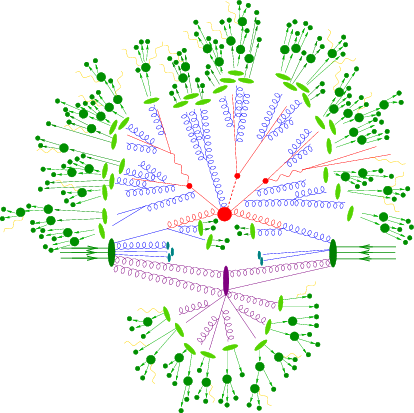
\includegraphics[width=0.5\textwidth]{Figures/collision.png}
		%\rule{35em}{0.5pt}
	\caption[A drawing of a proton-proton collision with its decay products.]{Drawing represents a proton-proton collision production a ttH event. The hard interaction, represented with big red circle, is followed by the decay of both top quarks and the Higgs boson. Additional hard QCD radiation and a secondary interaction, shown in red and purple, take place before the final-state partons hadronise (light green) and hadrons decay (dark green). Photon radiation is shown in yellow and it can occur at any stage \cite{Gleisberg:2008ta}. }
	\label{fig:collision}
\end{figure}


%-----------------------------------
%	SUBSECTION 2.1
%-----------------------------------

\subsection{Cross sections at hadron colliders}
\label{subsec:2.1}

	Determining cross sections for processes at hadron collides is not an easy task. The proton is a composite object consisting of partons, thus it is necessary to include its internal structure as well as the diagrams for the hard scattering process of interest. Quarks and gluons within the proton interact through strong force and are described using quantum chromodynamics. Calculations within QCD are possible thanks to \textit{asymptotic freedom} and \textit{factorization theorem}. Since the strong force coupling constant $\alpha_s$ depends on the scale of the process, for high momentum transfers ($Q >> \Lambda_{QCD}\approx 200$ MeV) it becomes sufficiently small to make perturbative expansion in $\alpha_s$ possible. This feature is called \textit{asymptotic freedom} and it is used to determine the hard process cross section. Figure \ref{fig:alpha_s} shows the results of the $\alpha_s$ measurements which is in complete agreement with the QCD predictions of asymptotic freedom. \\
\begin{figure}[htbp]
	\centering
		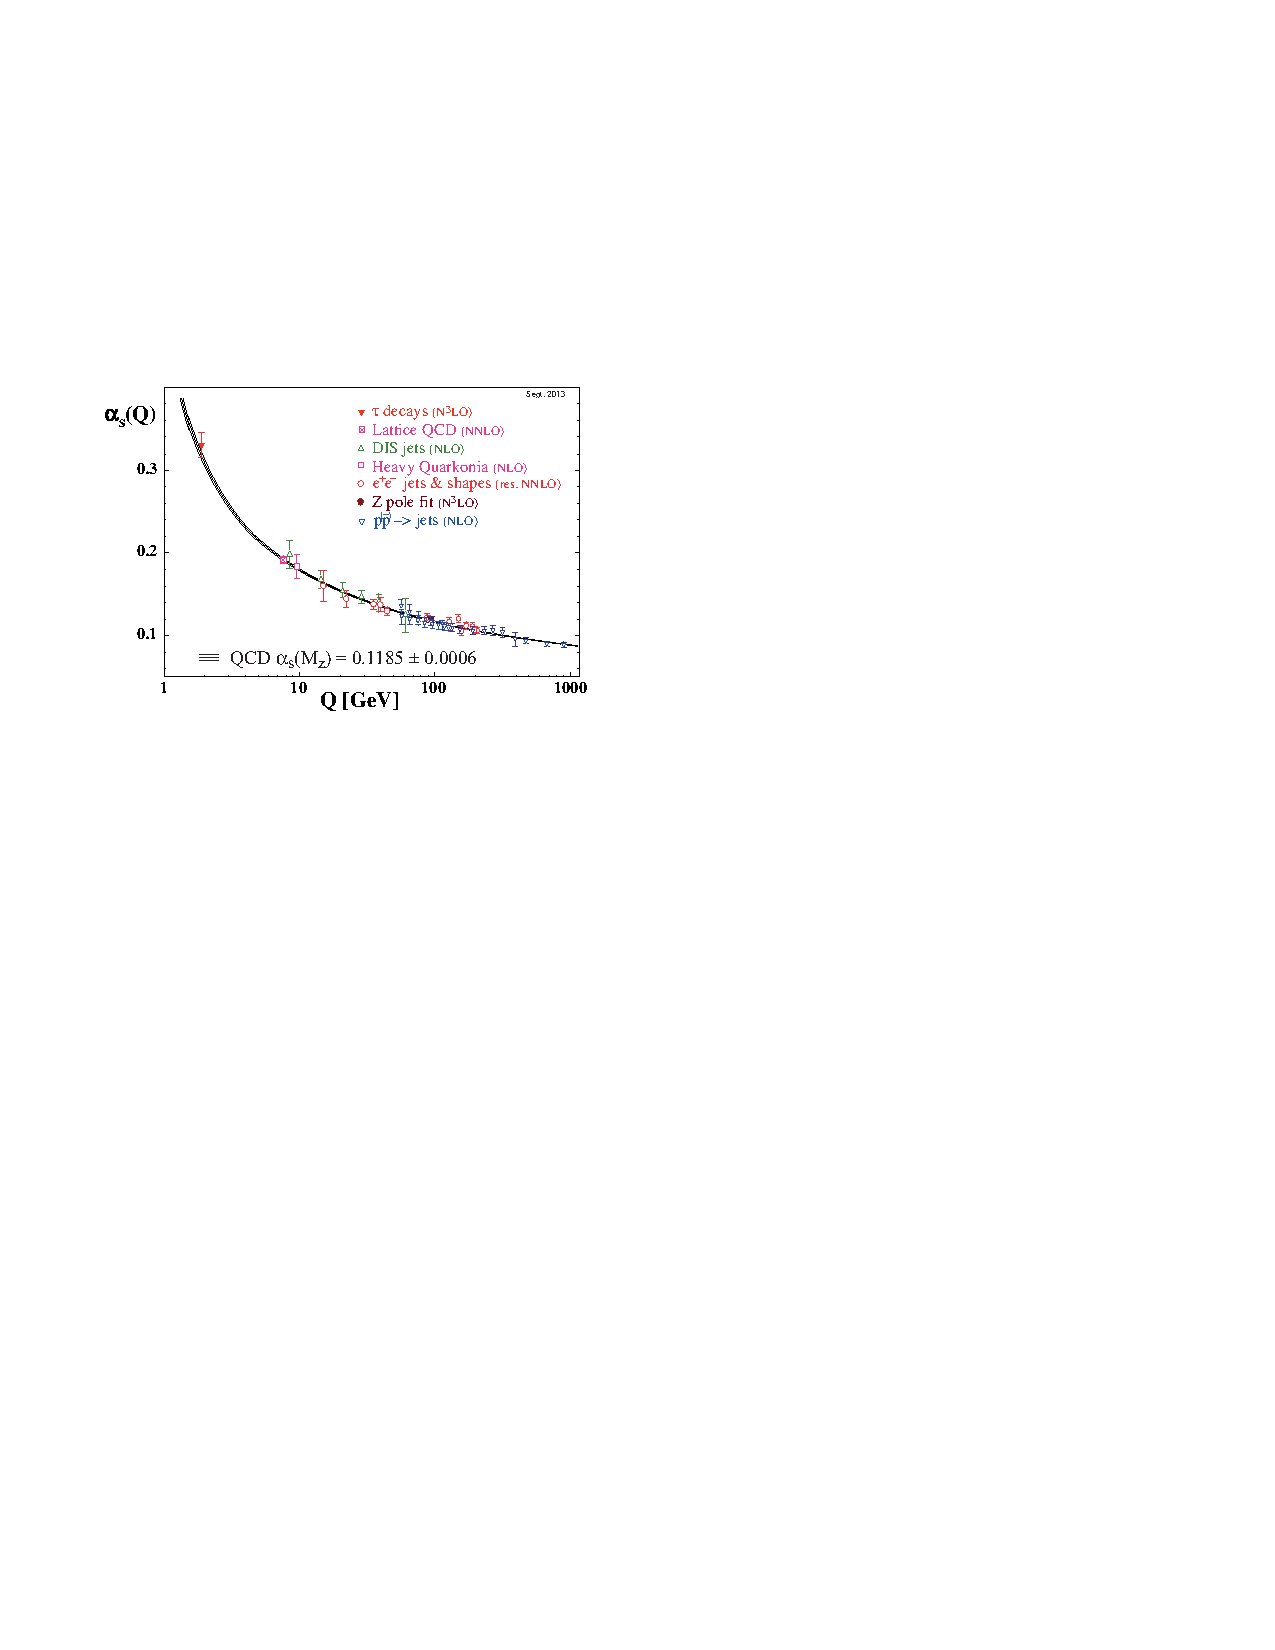
\includegraphics{Figures/alpha_s.pdf}
		%\rule{35em}{0.5pt}
	\caption[Strong force coupling constant]{Summary of measurement of strong coupling constant $\alpha_s$ as a function of momentum transfer\cite{Agashe:2014kda}. }
	\label{fig:alpha_s}
\end{figure}

	\par The \textit{ factorization theorem} is introduced to separate the two contributions in the cross section calculation, the contribution from the hard process calculated using perturbative QCD and the contribution from the internal structure of the proton. This means that hard scattering between partons is independent from the proton internal structure. The factorization scale is introduced as a cut-off below which perturbative QCD calculation cannot be performed.  Scale dependence of the strong coupling constant causes the hard and soft part of the process to happen at different time scales. 
	\begin{figure}[htbp]
	\centering
		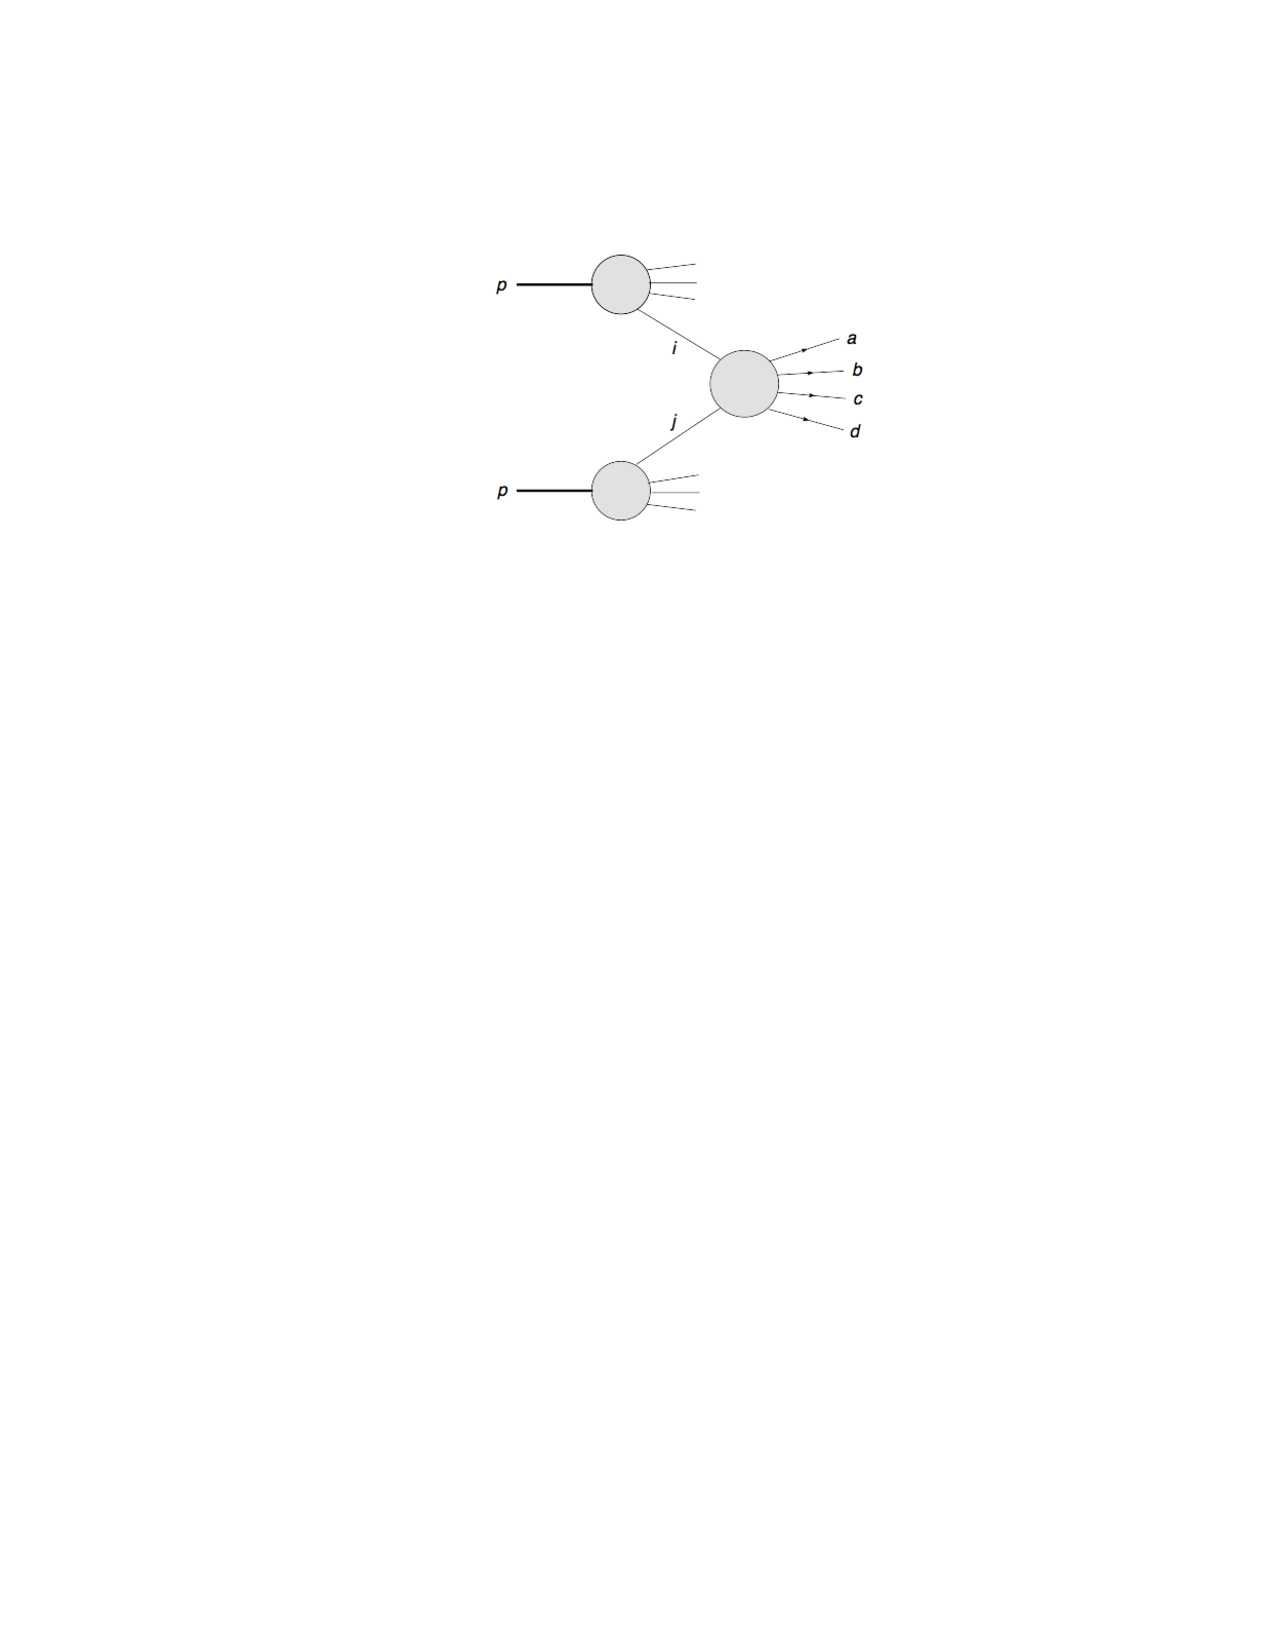
\includegraphics{Figures/diagram.pdf}
		%\rule{35em}{0.5pt}
	\caption[Drawing of a proton-proton collision]{Drawing of a proton-proton collision.}
	\label{fig:pp_drawing}
\end{figure}
The calculation the cross section for a process with two protons in the initial state and some interesting final state which we call X requires the following steps (as described in \cite{Campbell:2006wx}):
\begin{enumerate}
	\item Identify the leading order partonic processes that contribute to X
	\item Calculate the corresponding hard scattering cross section
	\item Determine the appropriate PDFs for initial state partons
	\item Make a specific choices for factorization($\mu_F$) and renormalization($\mu_R$) scales
	\item Perform integration over the fraction of momentum available for a given parton(x)  
\end{enumerate}
The cross section at hadron collides is thus a convolution of the hard scattering perturbative cross section and two incoming parton distribution functions.
\begin{equation}
\sigma_{AB} = \sum\limits_{n=1}^{\infty} \alpha_{s}^{n}(\mu_{R}^2)\sum\limits_{i,j} \int dx_1 dx_2 f_{i/A}(x_1,\mu_{F}^2) f_{j/B}(x_2,\mu_{F}^2) \sigma_{ij \rightarrow X}^{(n)}(x_1 x_2s,\mu_{R}^2,\mu_{F}^2)
 \label{eq:xsec}
\end{equation} 	

\par Equation \ref{eq:xsec} shows cross section perturbation series in $\alpha_s$, $n$ denotes the order of the series where $n=1$ is leading order, $n=2$ is next to leading order, etc. 
Hard process cross section between two partons $\sigma_{ij \rightarrow X}^{(n)}$ is computed in the framework of perturbative QCD and depends on $s$ which is the squared center of mass energy. 
Two functions denoted with $f_{i/A}$ and $f_{j/B}$ correspond to the probability density that parton $i$($j$) with proton momentum fraction $x_1$($x_2$) will be found inside a proton. and are called parton distribution functions (PDFs). These functions cannot be computed using perturbative QCD because momentum transfer values are small and the coupling constant becomes large. This phenomenon is called \textit{confinement} and it requires different treatment for the quarks inside the proton. The internal structure of a proton is described using parton distribution functions(PDF) which  are determined through deep inelastic scattering experiments. The sum over all combinations of partons has to be computed. The integral over available phase space for proton fraction momentum $dx$ is usually carried out numerically. 
Here $\mu_F$ represents the \textit{factorization scale} and $\mu_R$ is the \textit{renormalization scale} for running coupling constant. They are arbitrary cut-offs used to remove nonperturbative effects and be able to make perturbative calculations. If the cross section is computed in full series, $\mu_F$ and $\mu_R$ should cancel out, and the scale dependence should disappear. However, since fewer orders are used and some residual scale dependence is still present, this dependency can be used to estimate the contribution of the missing orders in the series.  
\par  The factorization scale controls soft and collinear emissions that can spoil the perturbative calculation. These emissions are then absorbed into the PDF for transverse momenta below $\mu_F$. Using DGLAP equations, PDFs can be evolved to any momentum transfer value which is described in detail in \cite{Campbell:2006wx}, and make the factorization cut-off possible. PDF evolutions are shown figure \ref{fig:MSTW} for one specific PDF function (MSTW) at momentum transfer values of $Q^2=10$ GeV$^2$ and $Q^2=10^4$ GeV$^2$ which corresponds to the typical momentum transfers for W boson production. At high momentum transfer values, sea quarks and gluons carry a much larger portion of the proton momentum and $b$ quark distributions become relevant.
\begin{figure}[htbp]
	\centering
		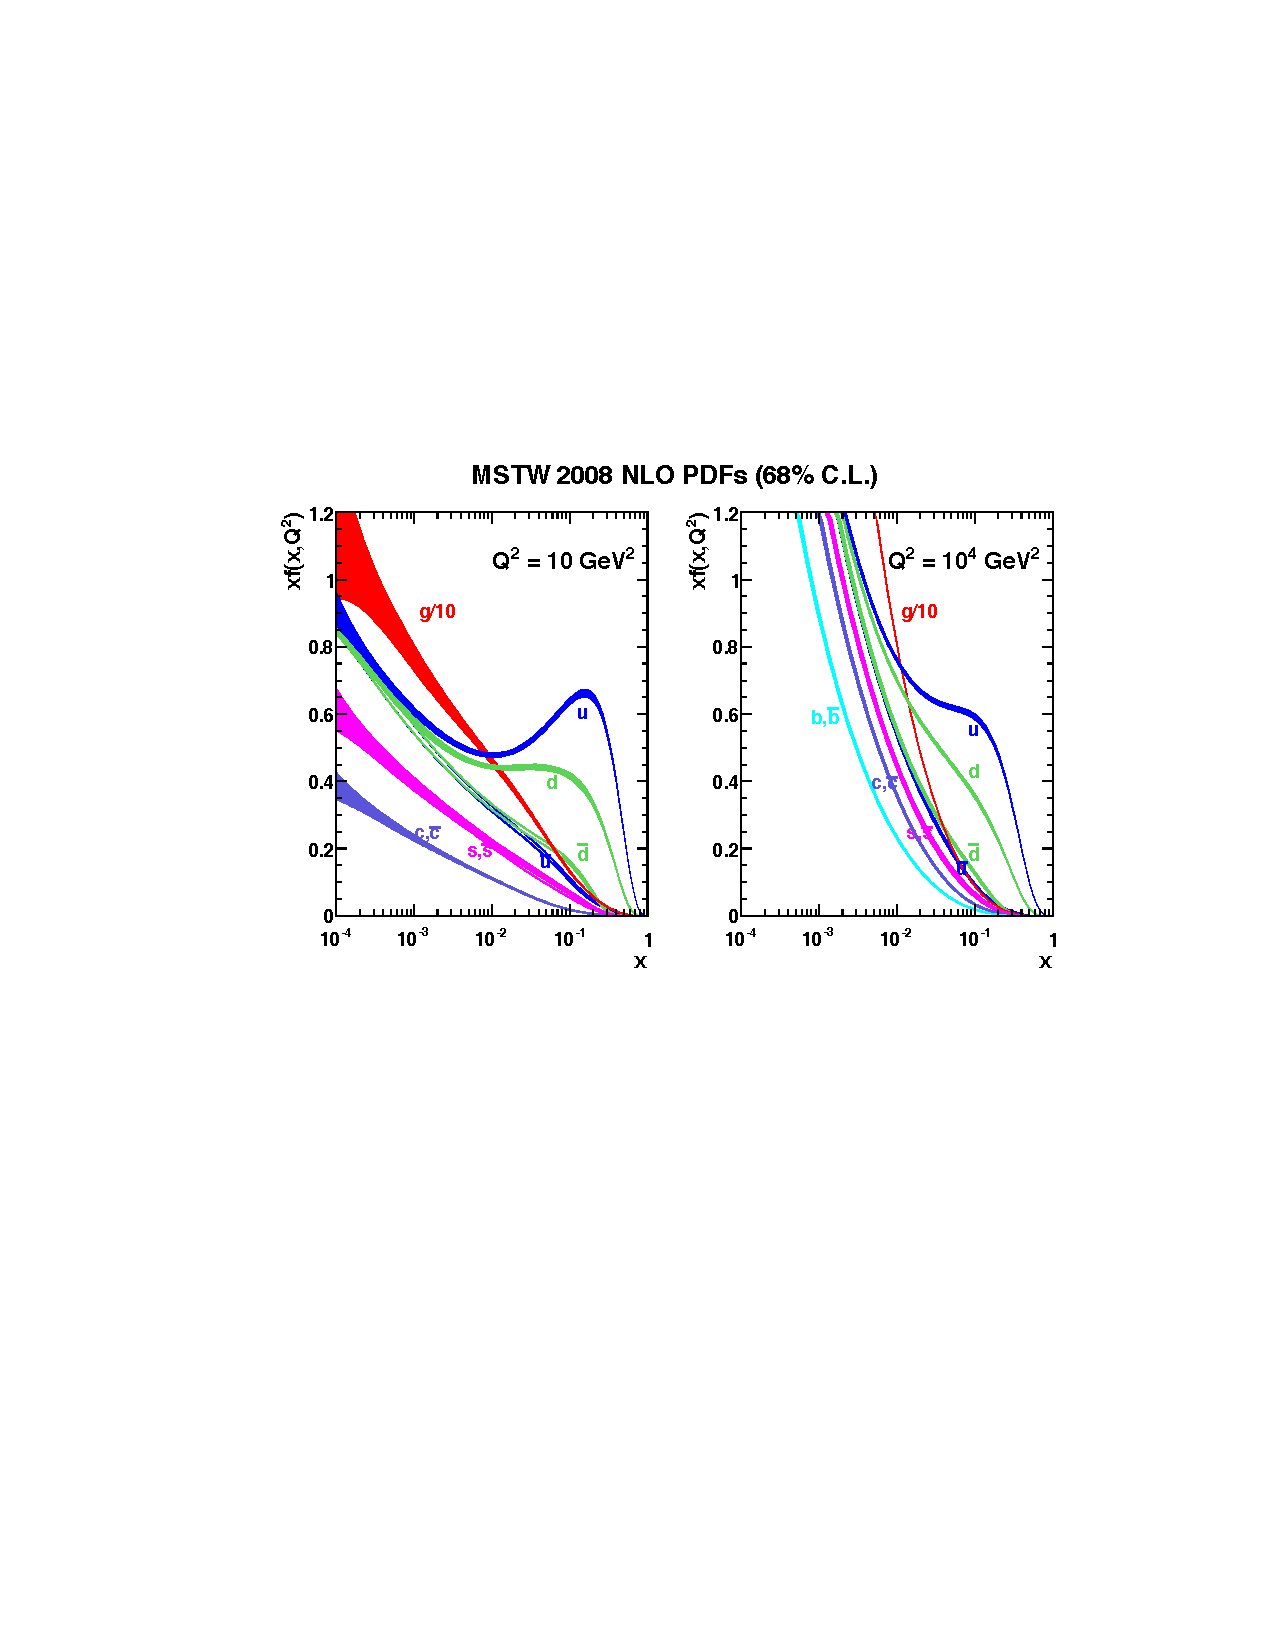
\includegraphics{Figures/MSTW.pdf}
		%\rule{35em}{0.5pt}
	\caption[Parton distribution functions for different momentum transfers]{Parton distribution functions calculated by the MSTW group for $Q^2=10$ GeV$^2$ (\textit{left}) and $Q^2=10^4$ GeV$^2$ (\textit{right}) \citep{Martin:2009iq}}
	\label{fig:MSTW}
\end{figure}	
The renormalization scale is another cut-off used to control divergences from the integration of high momentum loops in parton cross sections. If the momenta are larger than $\mu_R$, the divergences are absorbed in a redefined coupling constant $\alpha_s$ and the cross section calculation becomes finite. This approach is common in renormalizable field theories. However, such result depends on the renormalization scale and the resulting dependency can be calculated using renormalization group equation (RGE) \cite{opac-b1131978}.
\par Usually the factorization and renormalization scales are chosen to be identical and close to the scale of the process in question ($\mu_F=\mu_R=\mu_0\approx Q$). The choice of the scale in the case of W boson production is usually around the mass of the W boson. Taking into account specific kinematical properties of each event, a dynamic scale can be defined, for example $\mu^2_0=m_w^2+p_{T,W}^2$. In case of W boson and b jets production, adding the b quark mass or transverse momentum to the scale is also a viable option. 

\begin{figure}[htbp]
	\centering
		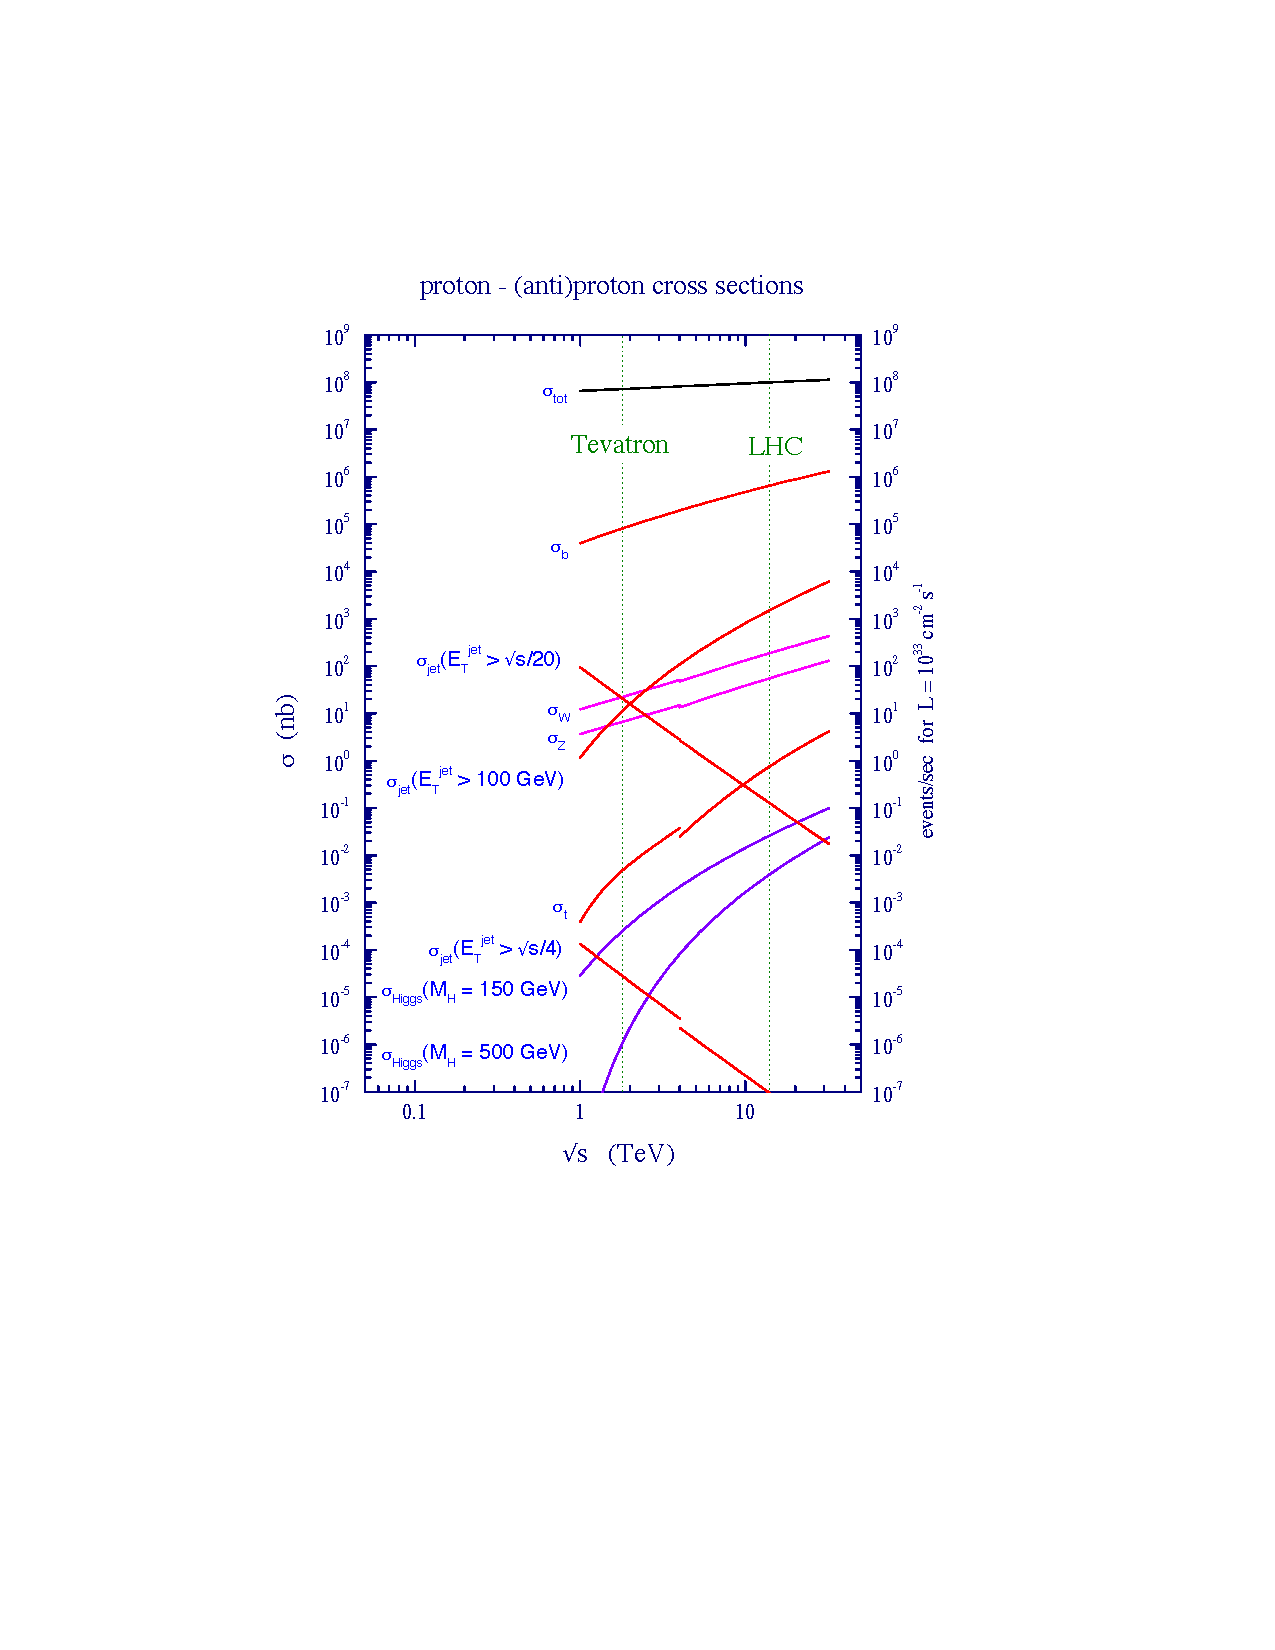
\includegraphics[width=0.7\textwidth]{Figures/pp_xsec.pdf}
		%\rule{35em}{0.5pt}
	\caption[Proton-proton cross sections]{Standard model cross sections as a function of center of mass energy.\cite{Campbell:2006wx} }
	\label{fig:pp_xsec}
\end{figure}
\par Figure \ref{fig:pp_xsec} shows some interesting standard model cross sections in proton-proton and proton-antiproton collisions as a function of a the center of mass energy. All cross sections have been computed to the NLO order in QCD using the above described procedure.

 
%-----------------------------------
%	SUBSECTION 2.2
%-----------------------------------

\subsection{Contributions to Wbb cross section}


From the theoretical point of view, calculations of W+b jets processes can be divided into two categories:
\begin{itemize}
\item only light quarks in the initial state shown in figure \ref{fig:LO_diag} - four flavour scheme (4FS)
\item b quark in the initial state shown in Figure \ref{fig:5FS_diag} - five flavor scheme (5FS) 
\end{itemize}
An additional contribution to Wbb production at hadron colliders comes from double parton interactions where a W boson and a pair of b quarks is produced in different hard process inside the same collision as shown in Figure \ref{fig:DPS_diag}. This contribution will be discussed in Section \ref{sec:DPS}.

\par The rationale behind using 4FS or 5FS is discussed in detail in \cite{Maltoni:2012pa}. The four flavor scheme approach assumes that bottom quarks are heavy and can only be created as pairs in collisions with high momentum transfer or as a decay product of t quark. Heavy quarks are not included in the initial state and their parton distribution function is set to zero, which means an effective theory is created where heavy quarks do not enter the computation of running coupling and the evolution of PDFs. If it happens that the scale of the process is much higher than the mass of the b quark, for example in the production of massive bosons, large logarithms of the type $log(Q^2/m_b^2)$ appear and can spoil the convergence of a fixed order perturbative expansion and introduce a large scale dependence into the final result. In the five flavor scheme calculations include b quark in the initial state allowing for some new and simpler processes to become available. These calculations allow ressumation of possibly large logarithms of type $log(Q^2/m_b^2)$ into the b quark parton distributions function possibly transforming some higher order calculations into much simpler leading order calculations.  
The result in \cite{Maltoni:2012pa} shows that at the LHC 4-flavor calculations are well behaved and two schemes are in good agreement. The typical size of the possibly problematic logarithms in four flavor scheme at hadron colliders is not large enough to spoil convergence. On the other hand, five flavor scheme is less dependent on the scale of the process and show smaller uncertainties which is in general very good for predictions of inclusive observables like the total cross section.  

\par First leading order calculations for associated production of a W boson and heavy quarks at hadron colliders were presented in 1993 \cite{Mangano:1992kp}. Feynmann diagram for leading order W + 2 b jets production is shown in figure \ref{fig:LO_diag}. Exact leading order matrix element has been computed and higher order corrections were estimated using Monte Carlo. Their results are summarized in the Figure \ref{fig:scale_dep} where the differential cross section for W+2 b jets as a function of the leading b jet $p_T$ is shown. Two scale choices have been studied, the first one with $\mu_0=M_{bb}$, which is the invariant mass of the dijet system and is represented with a solid line. The second choice is $\mu_0=m_W+p_T^W$ and is represented with the dotted line. Looking at the normalizations of two diagrams, the difference is clearly visible which indicates a strong dependence of the total cross section scale. However, the shape of the differential cross section shows the same behavior in both cases, which means that the scale only affects the total cross section.      
\begin{figure}[htbp]
	\centering
		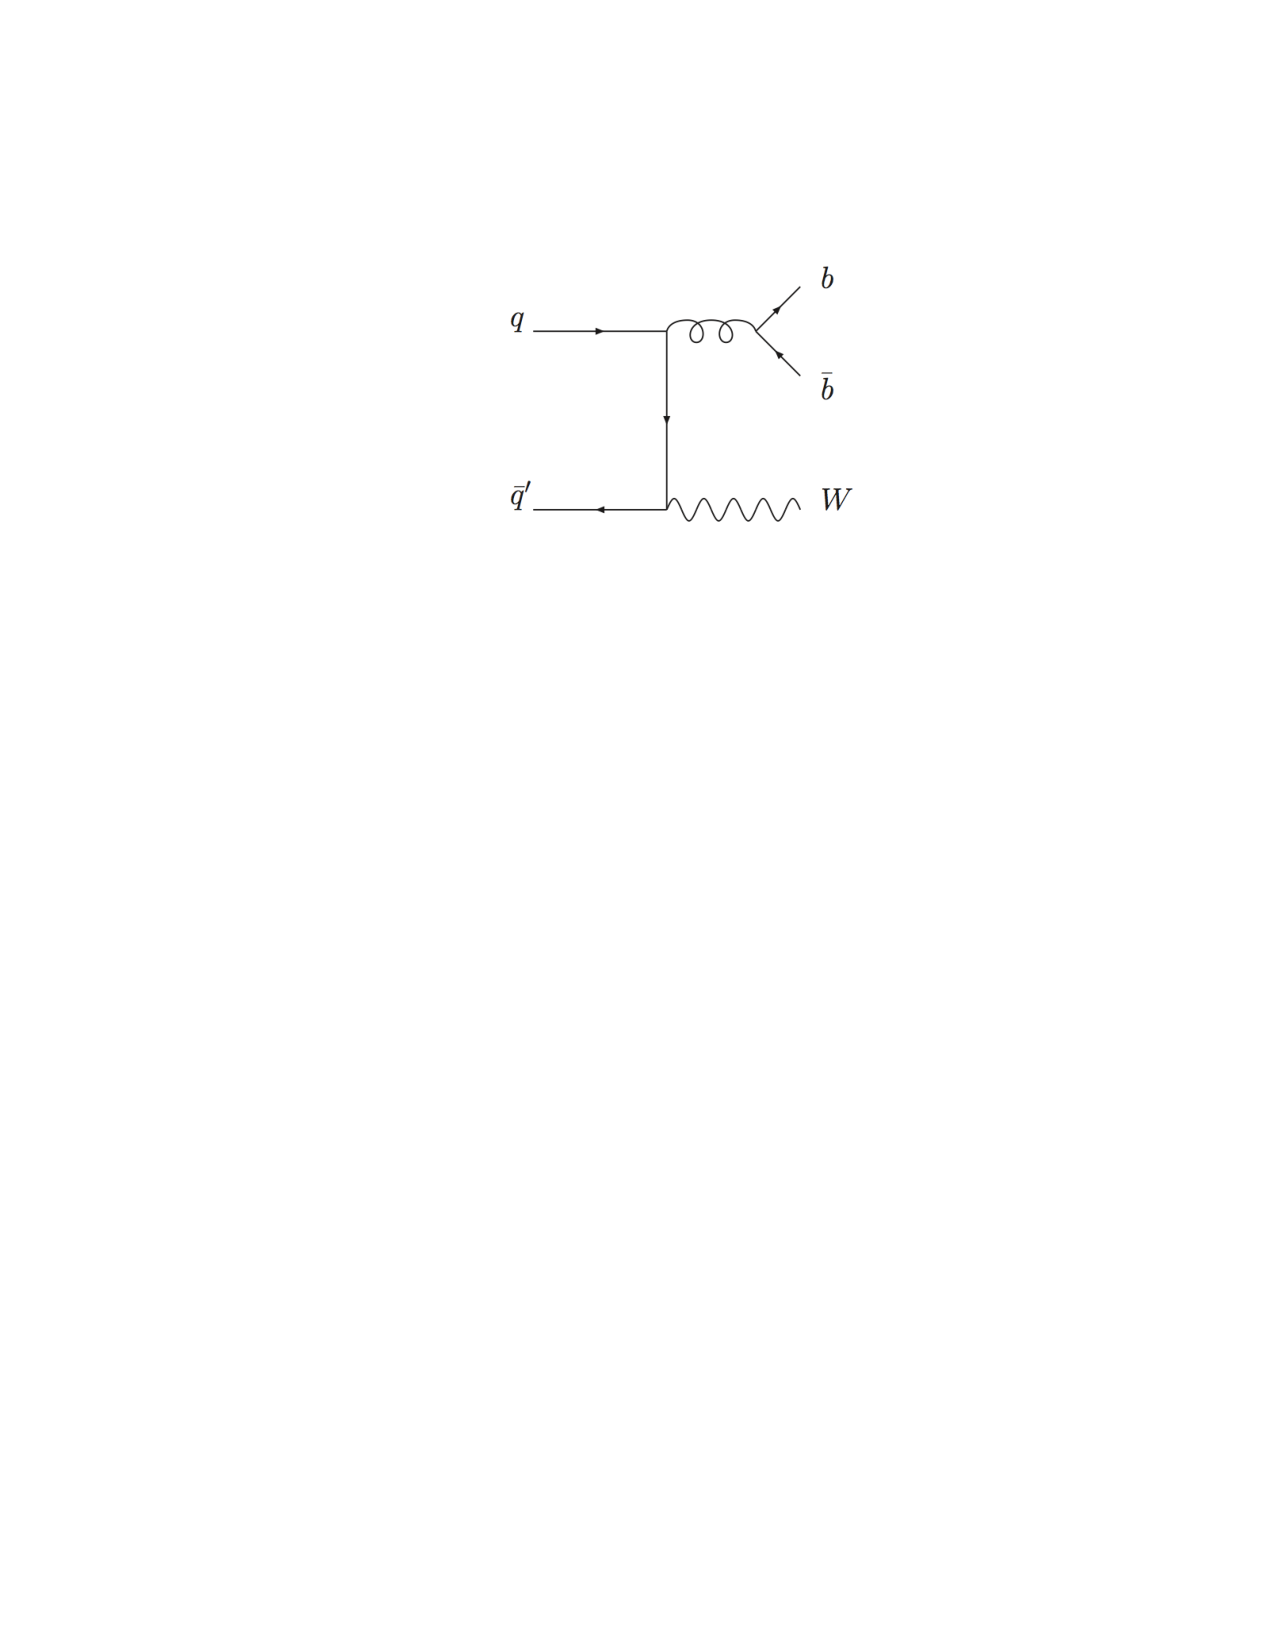
\includegraphics[width=0.5\textwidth]{Figures/LO_diag.pdf}
		%\rule{35em}{0.5pt}
	\caption[Leading order Wbb Feynmann diagram]{Leading order Wbb Feynmann diagram}
	\label{fig:LO_diag}
\end{figure}
\begin{figure}[htbp]
	\centering
		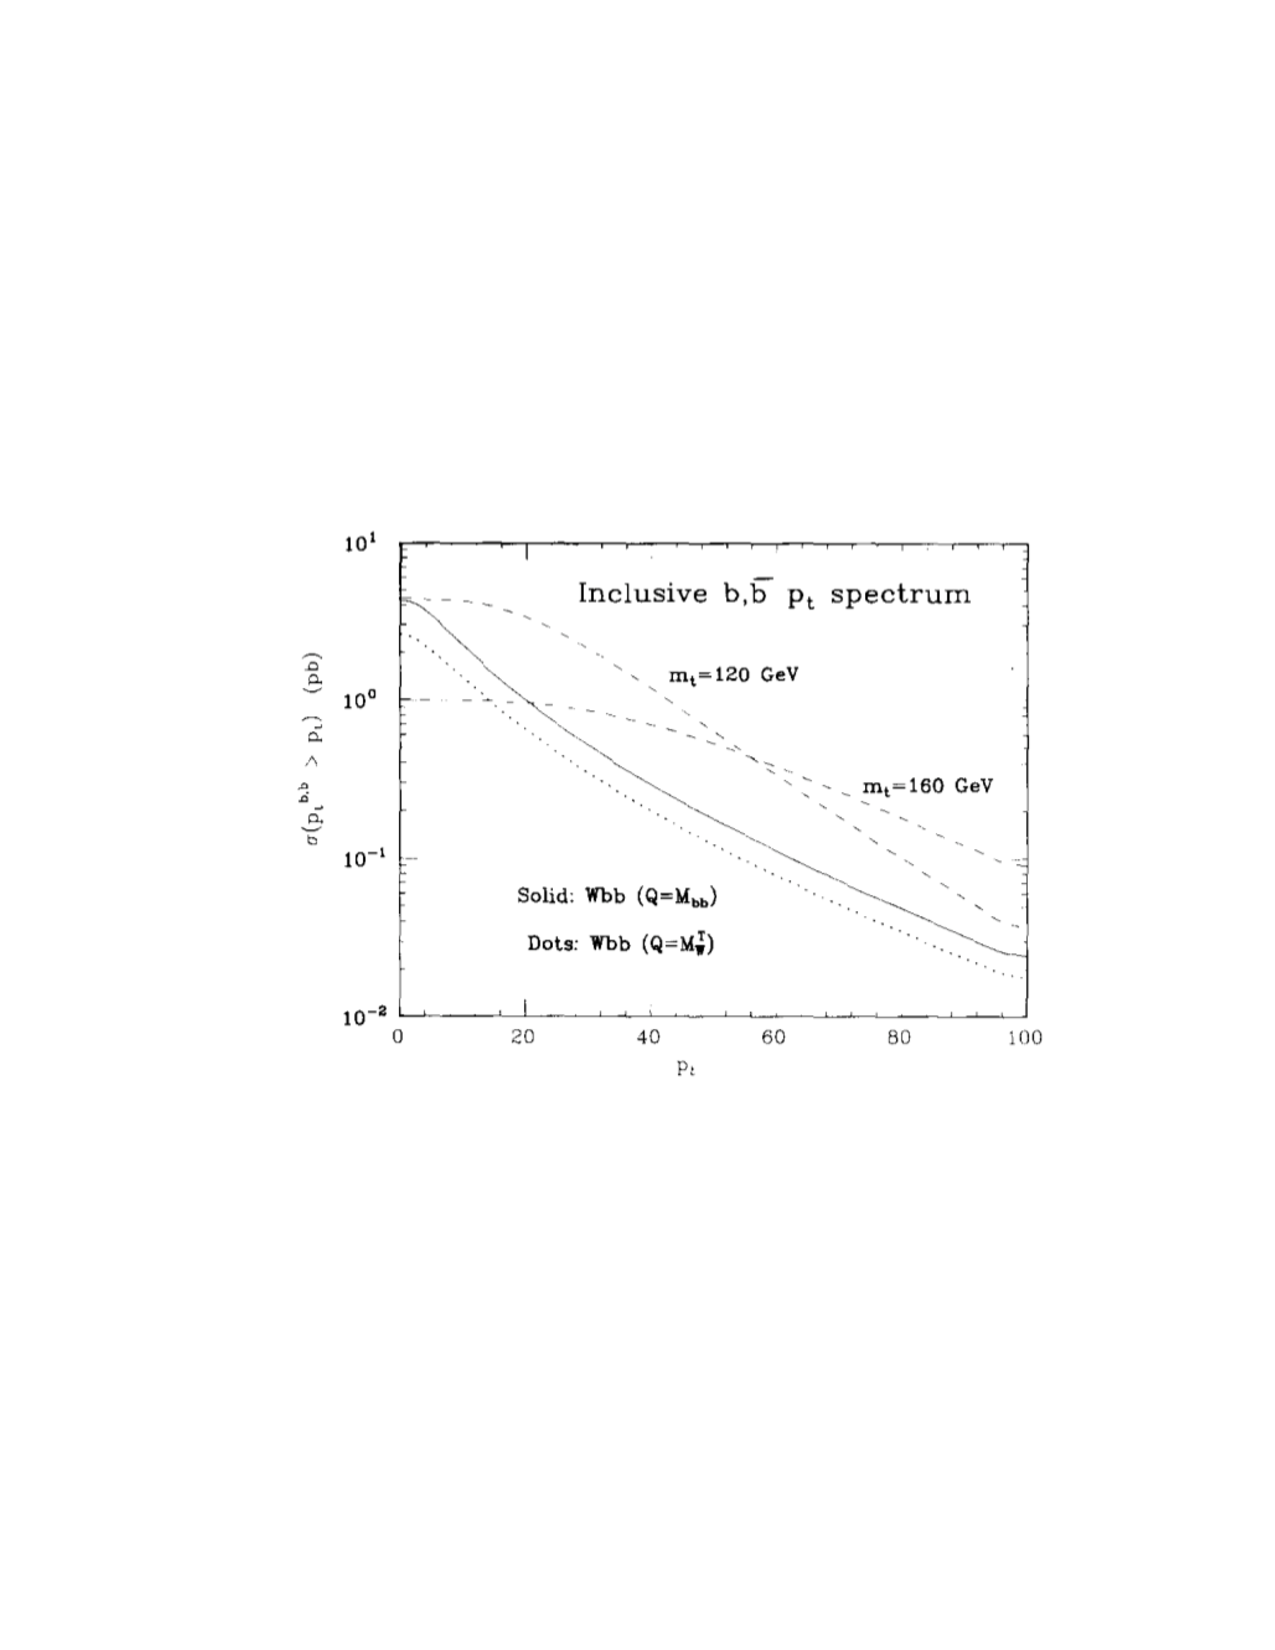
\includegraphics[width=0.7\textwidth]{Figures/scale_dep.pdf}
		%\rule{35em}{0.5pt}
	\caption[Scale dependence of Wbb cross section]{Scale dependence of Wbb cross section \cite{Mangano:1992kp}.}
	\label{fig:scale_dep}
\end{figure}
\par Later development of theoretical calculations was strongly motivated by reducing the scale dependence of the result and it included adding additional partons to the final state. This was a first step towards the full NLO calculation. The only thing missing was to take into account the loop effects. This approach made it possible to access some previously inaccessible kinematics, however at the expense of introducing additional scale dependence. The list of new final states is simple and it includes $Wb\bar{b}q$, $Wb\bar{b}q\bar{q}$, $Wb\bar{b}\bar{q}q'\bar{q'}$... For the measurements at the LHC in particular, calculations for new initial states $qg$ and $gg$ were of great importance. First results for W+2 jets were published in \cite{Ellis:1998fv}. Additional calculations were shown in \cite{Mangano:2001xp} for up to six additional jets in the final state. Although these processes are suppressed by an additional $\alpha_s$ factor, the gluon PDF inside a proton is much larger than anti-quark. This production mechanism is therefore significant at the LHC energies. 
\par First full NLO calculations were published in 2006 \cite{FebresCordero:2006sj}. 
Events with b jet pair in the final state were selected, with momentum of the dijet system $p_T>$15 GeV  and a pseudorapidity less than 2. Results were shown for two categories, inclusive and exclusive, depending on the treatment of extra jets. In the inclusive case events with additional jets were included, while in the exclusive case exactly two jets were required.
Figure \ref{fig:2006_scale} shows the overall scale dependence of LO, NLO inclusive and NLO exclusive total cross-sections, when both renormalization scale and factorization scale are varied independently between $\mu_0/2$ and $4\mu_0$ (with $\mu_0 = m_b + M_W /2)$, including full bottom-quark mass effects. NLO cross sections have a reduced scale dependence over most of the range of scales shown, and the exclusive NLO cross-section is more stable than the inclusive one especially at low scales.
%This is consistent with the fact that the inclusive NLO cross-section integrates over the
%entire phase space of the $qg(\bar{q}g) \rightarrow \bar{b}bW + q(\bar{q})$ channels that are evaluated with NLO $\alpha_s$ and NLO PDF, but are actually tree-level processes and retain therefore a strong scale
%dependence. 
The effect of the b quark mass has been shown to affect the total NLO cross section on the order of approximately $8\%$. This is expected to be small when considering well separated jets.
\begin{figure}[htbp]
	\centering
		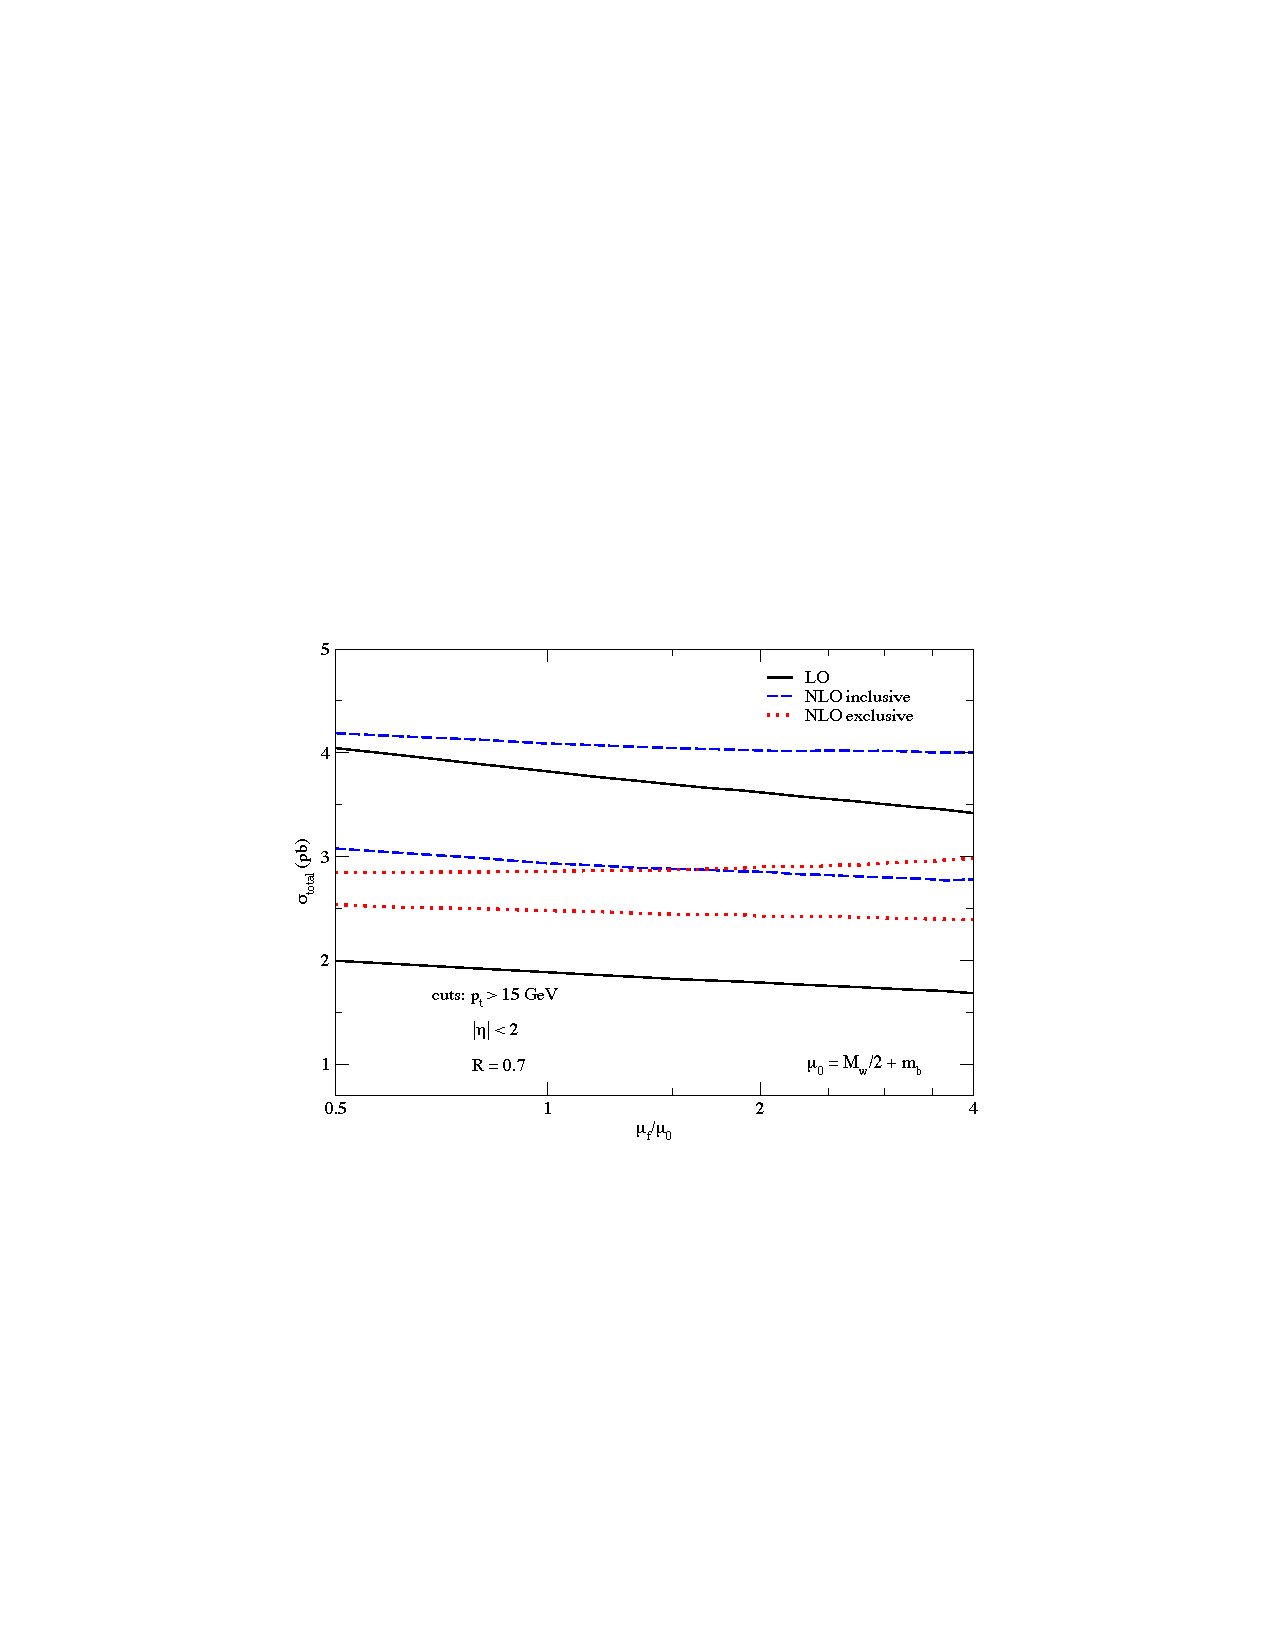
\includegraphics{Figures/2006_scale.pdf}
		%\rule{35em}{0.5pt}
	\caption[Wbb NLO scale dependence]{Wbb NLO scale dependence\cite{FebresCordero:2006sj}}
	\label{fig:2006_scale}
\end{figure}
\par New results published in 2007 explored in particular NLO corrections for events with W boson and two jets where at least one is b-tagged. It was shown that for LHC the correction factor is $\approx 1.9$. This paper was interesting in particular for its study of soft and collinear topologies, where two b quarks merge into one. Additionally, b quarks in the initial state were considered, giving rise to processes like $bq\rightarrow Wbq'$ shown in figure \ref{fig:5FS_diag}. The parton distribution function for b quark needed to be determined perturbatively using DGLAP equations. Another approach is to consider a gluon in the initial state, which then splits to $b\bar{b}$. 
\begin{figure}[htbp]
	\centering
		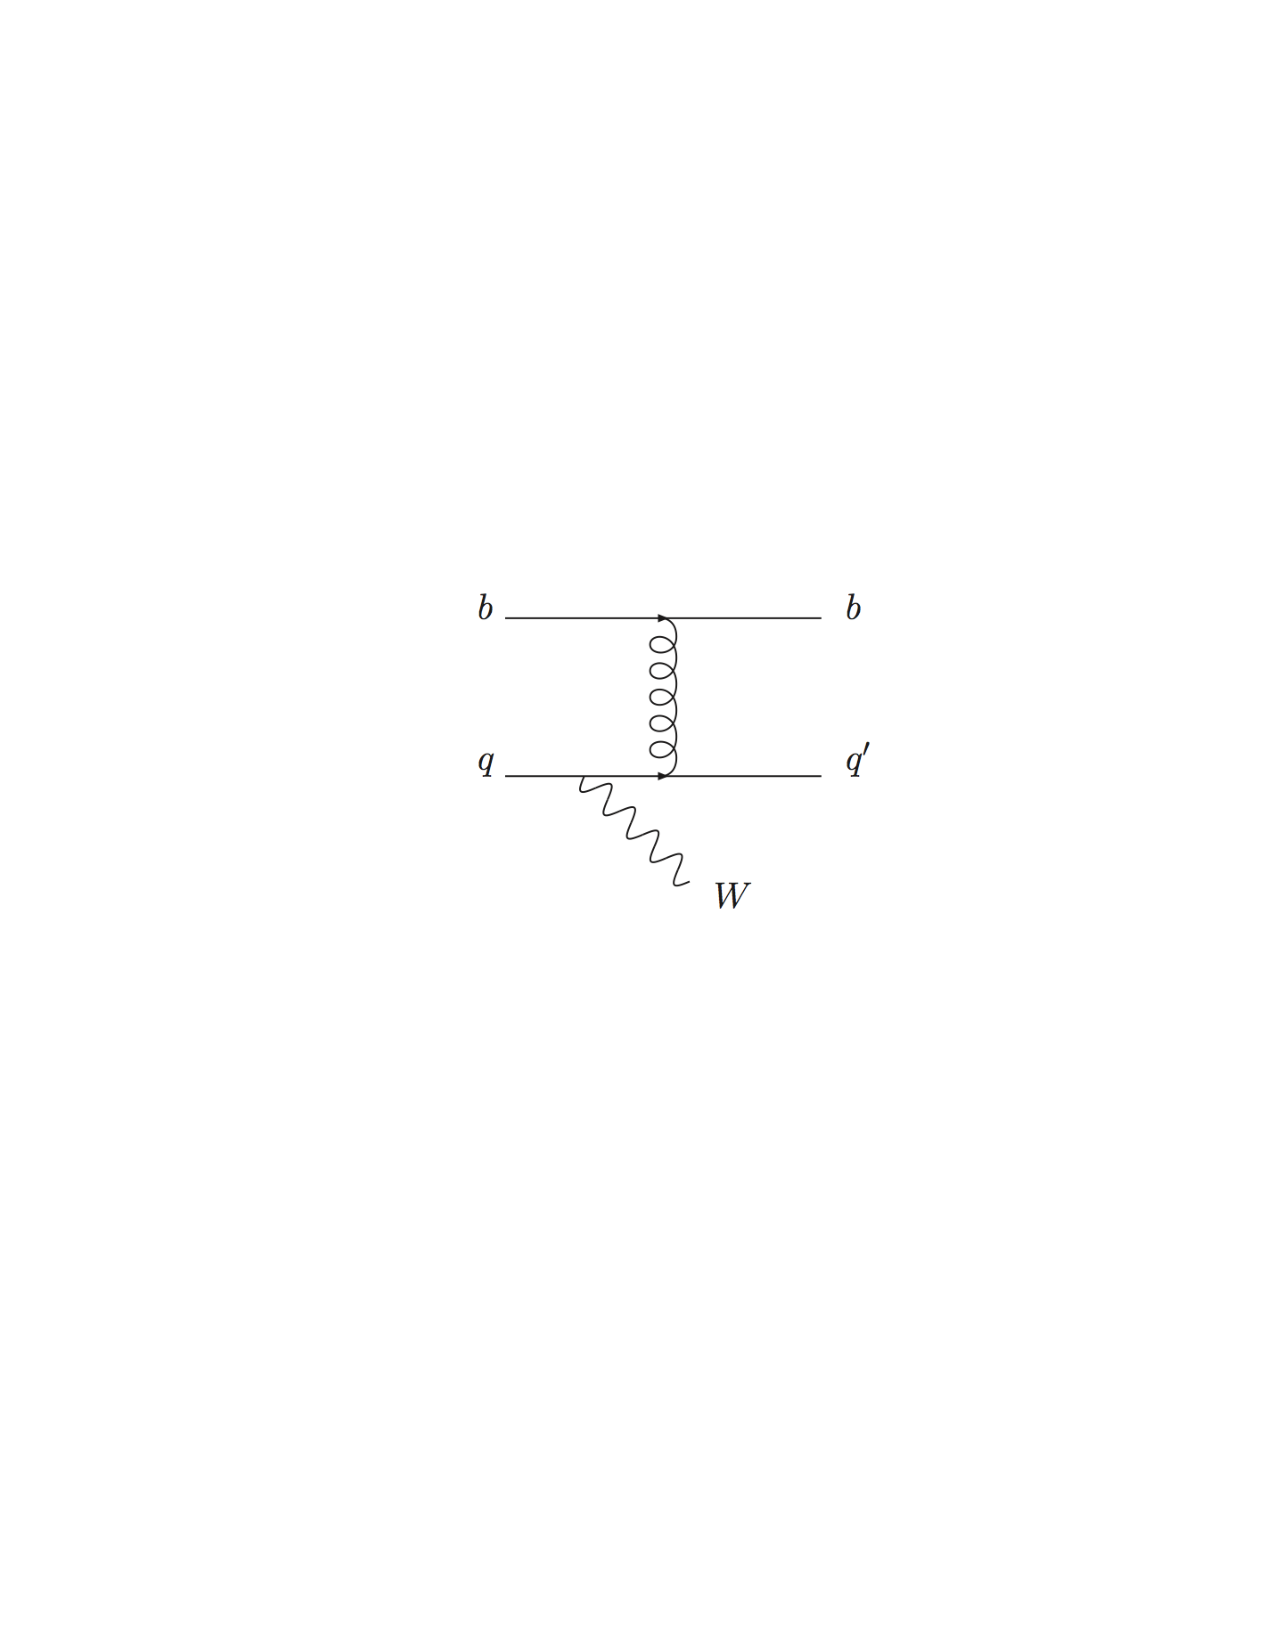
\includegraphics[width=0.5\textwidth]{Figures/5FS_diag.pdf}
		%\rule{35em}{0.5pt}
	\caption[Wbb production within 5 flavor scheme]{Wbb production within 5 flavor scheme}
	\label{fig:5FS_diag}
\end{figure}

\subsubsection{Double parton scattering}
\label{sec:DPS}

\par Multiple parton interactions happen due to the composite nature of the proton. Usually it is assumed that only one hard scattering occurs per bunch crossing. The probability of single parton interaction in hadron collisions is very small thus having two or more interactions is highly suppressed. However, sometimes it can happen that two such partons exist which results in two hard scatterings in the same collision. This phenomenon is called Double Parton Scattering (DPS) and is shown in Figure \ref{fig:DPS_diag}. In the framework of this thesis, two partons are responsible for the creation of a W boson and other two for creation of a pair of b jets. 
\begin{figure}[htbp]
	\centering
		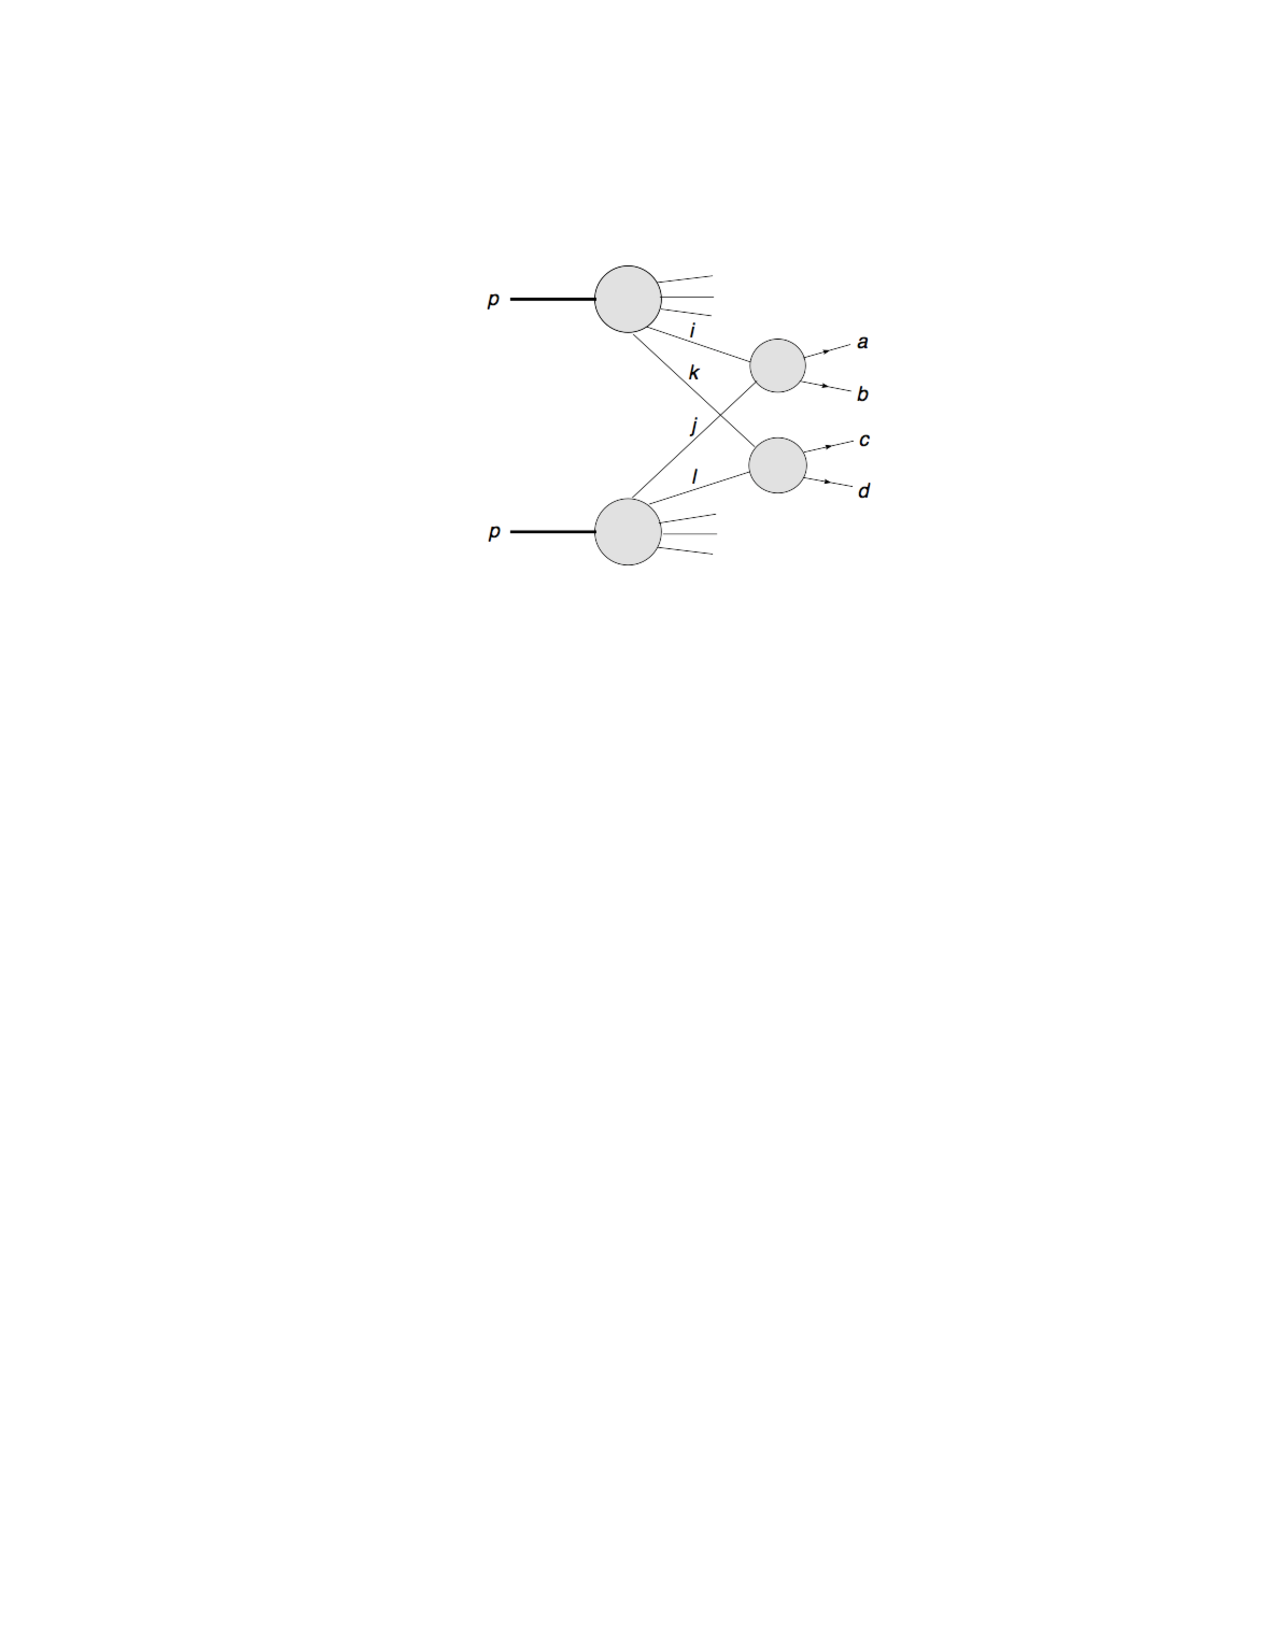
\includegraphics[width=0.5\textwidth]{Figures/DPS_diag.pdf}
		%\rule{35em}{0.5pt}
	\caption[Double parton scattering]{Double parton scattering}
	\label{fig:DPS_diag}
\end{figure}
\par Double parton scattering cannot be modeled in the framework of preturbative QCD, but it is approximated using simulations. The phenomenology of DPS starts from the assumption that factorization between the two hard processes is possible, as well as factorization between hard processes and proton kinematics. Cross sections for hard scatterings are computed separately for each pair of partons. However, instead of using regular parton distribution functions, a new set of distribution functions has been defined which are called Double Parton Distribution Functions (dPDFs). Factorized cross section for two hard processes A and B to happen in proton-proton scattering can be written as:
\begin{equation}
\begin{split}
\sigma_{(A,B)}^{DPS} \sim \sum\limits_{i,j,k,l} \int & dx_1 dx_2  dx'_1 dx'_2 d^2b  \Gamma_{ij}(x_1,x_2,b;Q_1,Q_2)\sigma_{ik}^A(x_1,x'_1) \\
 & \sigma_{jl}^B(x_2,x'_2) \Gamma_{kl}(x'_1,x'_2,b;Q_1,Q_2)
\end{split}
\end{equation}
\par Parton level cross sections are denoted with $\sigma_{ik}$, for hard process between partons $i$ and $k$, and $\sigma_{jl}$ for hard process between partons $j$ and $l$. These are the same as for single parton scattering and are known for most of the processes of interest today. The quantity $\Gamma_{ij}(x_1,x_2,b;t_1,t_2)$ represents the double parton distribution function, which describes the probability of finding a parton $i$ with momentum fraction $x_1$ at scale $Q_1$ inside a proton together with a parton $j$ with momentum fraction $x_2$ at scale $Q_2$. Another parameter in this distribution function is $b$, which describes the transverse distance between two partons. The scales $Q_1$ and $Q_2$ and correspond to characteristic scales of hard processes $A$ and $B$. For example in the framework of this thesis W boson production would correspond to process $A$ and production of two b jets would correspond to process $B$. This study is described in detail in \cite{Quackenbush:2011bf}. Usually, it is assumed that $\Gamma_{ij}(x_1,x_2,b;t_1,t_2)$ can be decomposed into two components, longitudinal and transversal in the following way:
\begin{equation}
\Gamma_{ij}(x_1,x_2,b;t_1,t_2) = D^{ij}_h(x_1,x_2;t_1,t_2)F_j^i(b)
\end{equation} 
The interpretation of the function $D^{ij}_h(x_1,x_2;t_1,t_2)$ within QCD is the probability of finding parton $i$ with scale $Q_1$ and parton $j$ with scale $Q_2$. These functions cannot be determined using perturbative QCD. Thus good modeling and to correctly take into account correlations between longitudinal momenta and transverse position is essential to making accurate cross section predictions. 
\par More details on how to determine dPDFs can be found in \cite{Gaunt:2009re}. In the simplest case $D^{ij}_h(x_1,x_2;t_1,t_2)$ can be taken as a product of single parton distribution functions taking into account effects like $x_1+x_2<1$. Since $F_j^i(b)$ is the only part of $\sigma_{(A,B)}^{DPS}$ that depends only on $b$, integration over b can be performed giving an effective cross section $\sigma_{eff}$ which is related to the size of the proton and can be seen as an effective area of the interaction. This approach yields a simplified expression for the double parton scattering cross section:
\begin{equation}
\sigma_{(A,B)}^{DPS} \sim \frac{1}{\sigma_{eff}} \sigma^{SPS}_{(A)} \sigma^{SPS}_{(B)}
\end{equation}
Here $\sigma^{SPS}_{(A)}$ and $\sigma^{SPS}_{(B)}$ are single parton scattering cross section which can be obtained using equation \ref{eq:xsec}.
\par However, this factorized approach does not take into account some simple correlations, e.g. between the probability to find a quark of some flavor and to find find another quark with the same flavor. While for some simple cases with low parton momentum fractions this factorized approach may give accurate results, for more complicated cases like calculating fiducial cross sections, acceptance cuts can spoil the equation. Thus, a simulation of the full kinematical effects is necessary.
\par First measurements of $\sigma_{eff}$ have been performed by the AFS collaboration at the ISR (CERN) which obtained $\sigma_{eff} \sim$ 5 mb at 63GeV. Both CDF and D0 collaborations at Tevatron reported $\sigma_{eff} \sim 15$ mb which is roughly 20$\%$ of the total $p\bar{p}$ cross section at Tevatron energies. Their data also show no sign of dependence on $x$ in measured $\sigma_{eff}$  in the accessible $x$ ranges. Later measurements performed by ATLAS ans CMS collaborations are in reasonable agreement with previous results. All results are summarized in Figure \ref{fig:DPS_res}.
\begin{figure}[htbp]
	\centering
		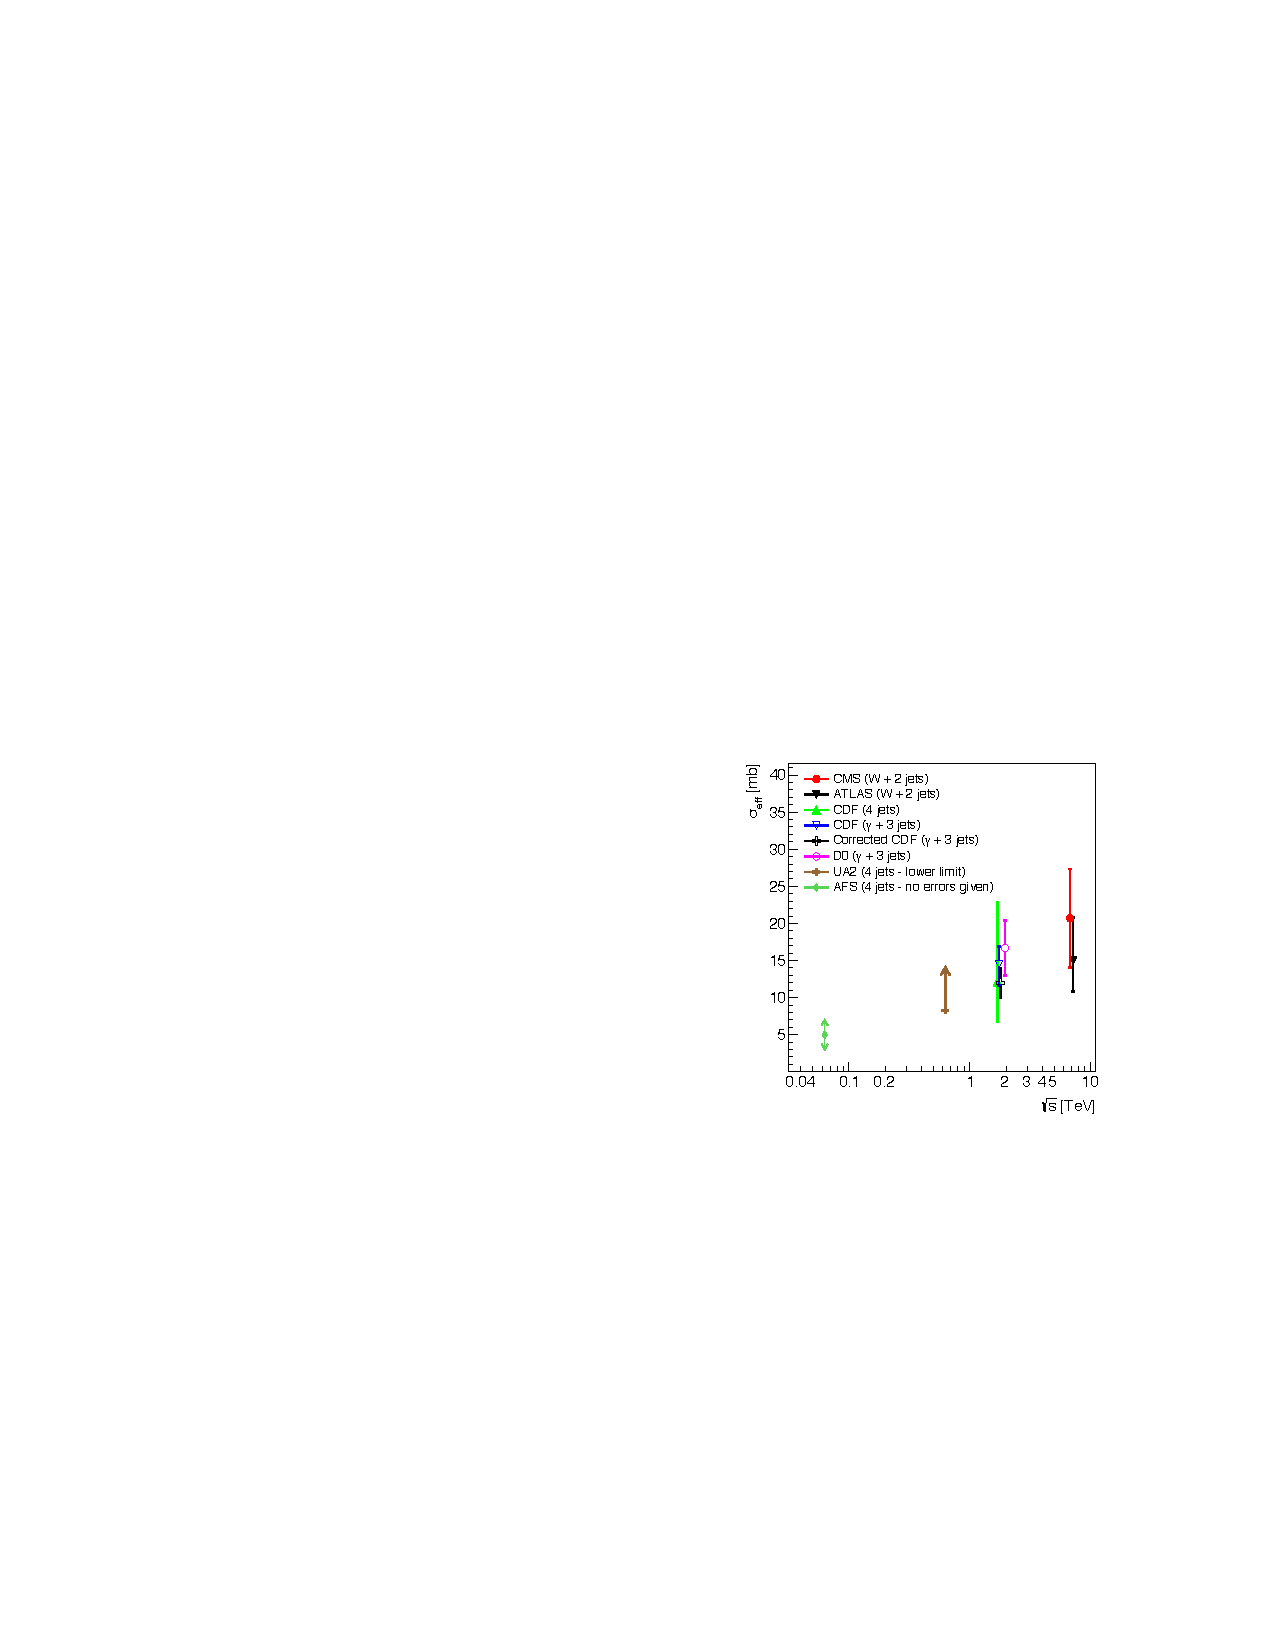
\includegraphics[width=0.6\textwidth]{Figures/DPS_res.pdf}
		%\rule{35em}{0.5pt}
	\caption[Results of $\sigma_{eff}$ measurements]{Center of mass energy dependence of $\sigma_{eff}$ as reported from different collaborations. All these measurements use different approaches to estimate $\sigma_{eff}$. \cite{Bansal:2014paa}}
	\label{fig:DPS_res}
\end{figure}
\par Double parton scattering measurement at CMS is performed by selecting events with a W + 2-jet final state where one hard interaction produces a W boson and another produces a dijet \cite{Chatrchyan:2013xxa}. The W + 2-jet process is attractive because the muonic decay of the W provides a clean tag and the large dijet production cross section increases the probability of observing DPS. Events containing a W + 2-jet final state originating from single parton scattering (SPS) constitute an irreducible background. Results were obtained by performing a template fit to two uncorrelated variables: the relative $p_T$ balance between two jets ($\Delta p_T$) and the angle between W boson and a dijet system. Obtained results again show that the contribution of DPS to the total cross section is $\sim 20\%$ which is in good agreement with previous Tevatron results. The DPS contribution in the case od W + 2 b jets is estimated to be $\sim 15\%$. \cite{Chatrchyan:2013uza}

%----------------------------------------------------------------------------------------
%	SECTION 2.3
%----------------------------------------------------------------------------------------

\section{Previous measurements}
\label{sec:2.3}
	\par Previous measurements of a W boson produced in association with b quarks have been performed on different experiments. However, the final states and phase space used in these measurements were different, which means that the results cannot be directly compared. They can nevertheless be compared with theoretical predictions. This process was measured for the first time at Tevatron with D0 and CDF experiments at $\sqrt{s} =$ 1.96 TeV. The CDF collaboration published its result in 2009 and the cross-section measured is that of “jets from b-quarks produced with a W boson” \cite{Aaltonen:2009qi}. The event selection is based on reconstructing a leptonically decaying W boson, and one or two jets where at least one has to be b-tagged. Events with jets from light quarks are vetoed with a cut on the secondary vertex mass. Contribution of other background events containing a b quark in the final state (e.g. events with top quark) is estimated using Monte Carlo simulations. The measured cross section is 2.8 standard deviations higher than the corresponding theoretical prediction. 
\par The D0 collaboration published their result in 2012. with a somewhat different phase space definition \cite{D0:2012qt}. The difference with respect to the CDF measurement consists in the inclusion of events with 3 jets and reduced pseudorapidity range in which the measurement was performed. The measurement technique is similar to that of CDF, although b-tagging algorithms were slightly different. The measured cross section was in good agreement with the standard model prediction.
\par	 First measurements at the LHC were published by the ATLAS collaboration based on 36 pb$^{-1}$ of integrated luminosity at $\sqrt{s} =$ 7 TeV. One year later they improved their measurement using $4.6$fb$^{-1}$ \cite{Aad:2013vka}. Selected events contain one reconstructed electron or muon, significant amount of missing transverse energy and one or two jets where exactly one is b-tagged. The phase space is divided in two regions, depending on the number of jets. Events with exactly 2 b jets and events with more than 2 jets are vetoed in order to suppress background events from top quark decay. The results are shown in Figure \ref{fig:atlas_tot}. The cross section measurement in the one jet region shows an excess corresponding to 1.5 standard deviations. In the two jet region, the measured cross section is in good agreement with theoretical predictions. A differential cross section measurement as a function of leading b jet transverse momentum has been performed for the first time. The results are shown in figure \ref{fig:atlas_diff}. The cross section measurement in the one jet region is again higher than NLO predictions but within theoretical and experimental uncertainties. The cross section measured for the events with two jets is in good agreement with the theoretical prediction.
\begin{figure}[htbp]
	\centering
		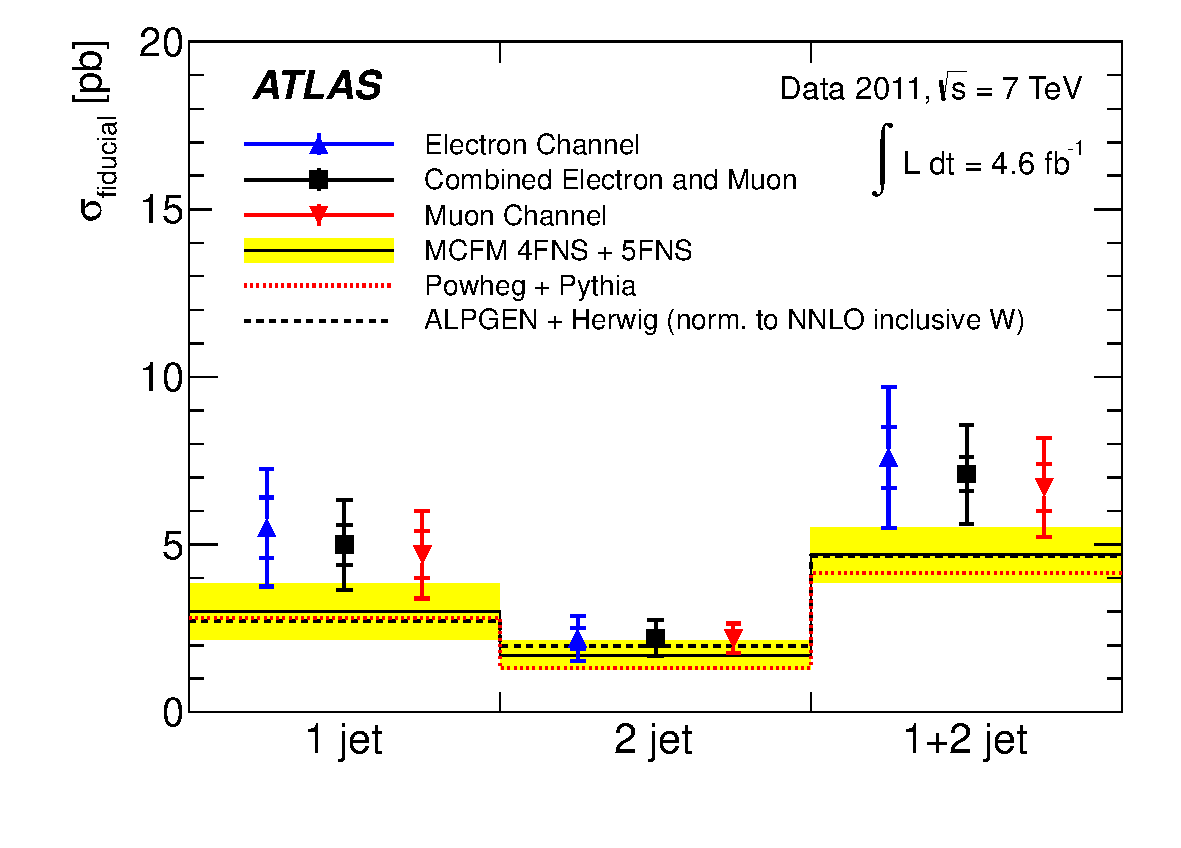
\includegraphics[width=0.7\linewidth]{Figures/atlas_total.pdf}
		%\rule{35em}{0.5pt}
	\caption[Atlas Wbb total cross section measurement]{Measured fiducial cross-sections in the electron, muon, and combined electron and muon channels. The cross-sections are given in the 1-jet, 2-jet, and 1+2-jet fiducial regions. \cite{Aad:2013vka} }
	\label{fig:atlas_tot}
\end{figure}
\begin{figure}
\centering
  \begin{subfigure}{.5\textwidth}
  	\centering
  	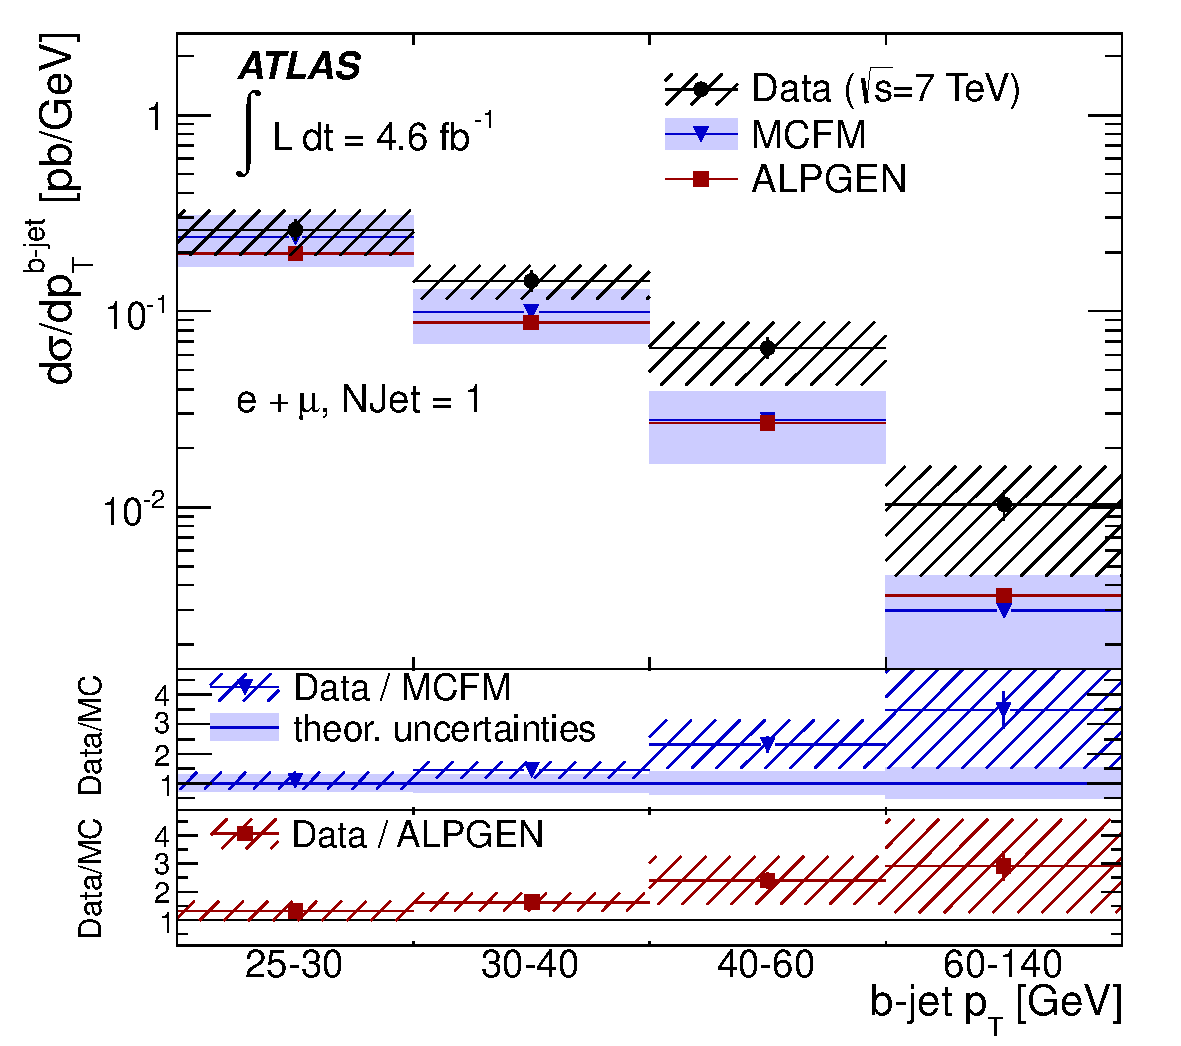
\includegraphics[width=\linewidth]{Figures/atlas_diff1j.pdf}
	\caption{}  
  	\label{fig:atlas_diff1j}
\end{subfigure}%
\begin{subfigure}{.5\textwidth}
  \centering
  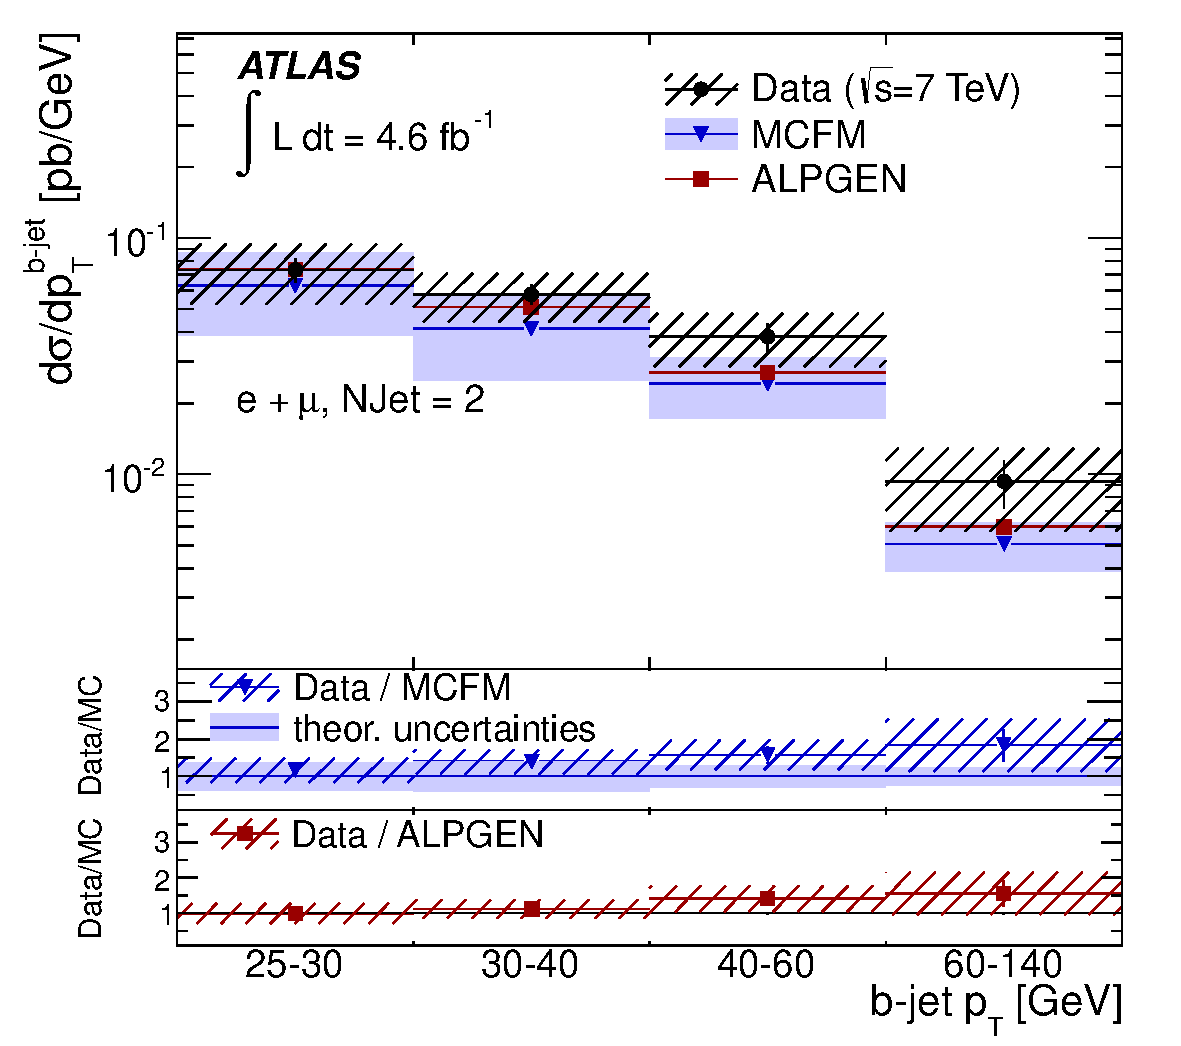
\includegraphics[width=\linewidth]{Figures/atlas_diff.pdf}
  \caption{}
  \label{fig:atlas_diff2j}
\end{subfigure}
\caption[Measured differential W+b-jets cross-sections as a function of leading b-jet $p_{T}$]{Measured differential W+b-jets cross-sections as a function of leading b-jet $p_{T}$ in the 1-jet (\ref{fig:atlas_diff1j}) and 2-jet (\ref{fig:atlas_diff2j}) fiducial regions, obtained by combining the muon and electron channel results. \cite{Aad:2013vka}}
\label{fig:atlas_diff}
\end{figure}		
\par The CMS collaboration published results corresponding to data collected during 2011 at 7 TeV corresponding to 5 fb$^{-1}$ of data. Selected events contained a muon and missing transverse energy in the final state, together with two b-tagged jets. All additional lepton and jet activity was vetoed to reduce the background contributions. Figure \ref{fig:cms_total} shows the leading jet transverse momentum distribution used for signal extraction. The measured cross section is in excellent agreement with the Standard model prediction. \cite{Chatrchyan:2013uza}

\begin{figure}[htbp]
	\centering
		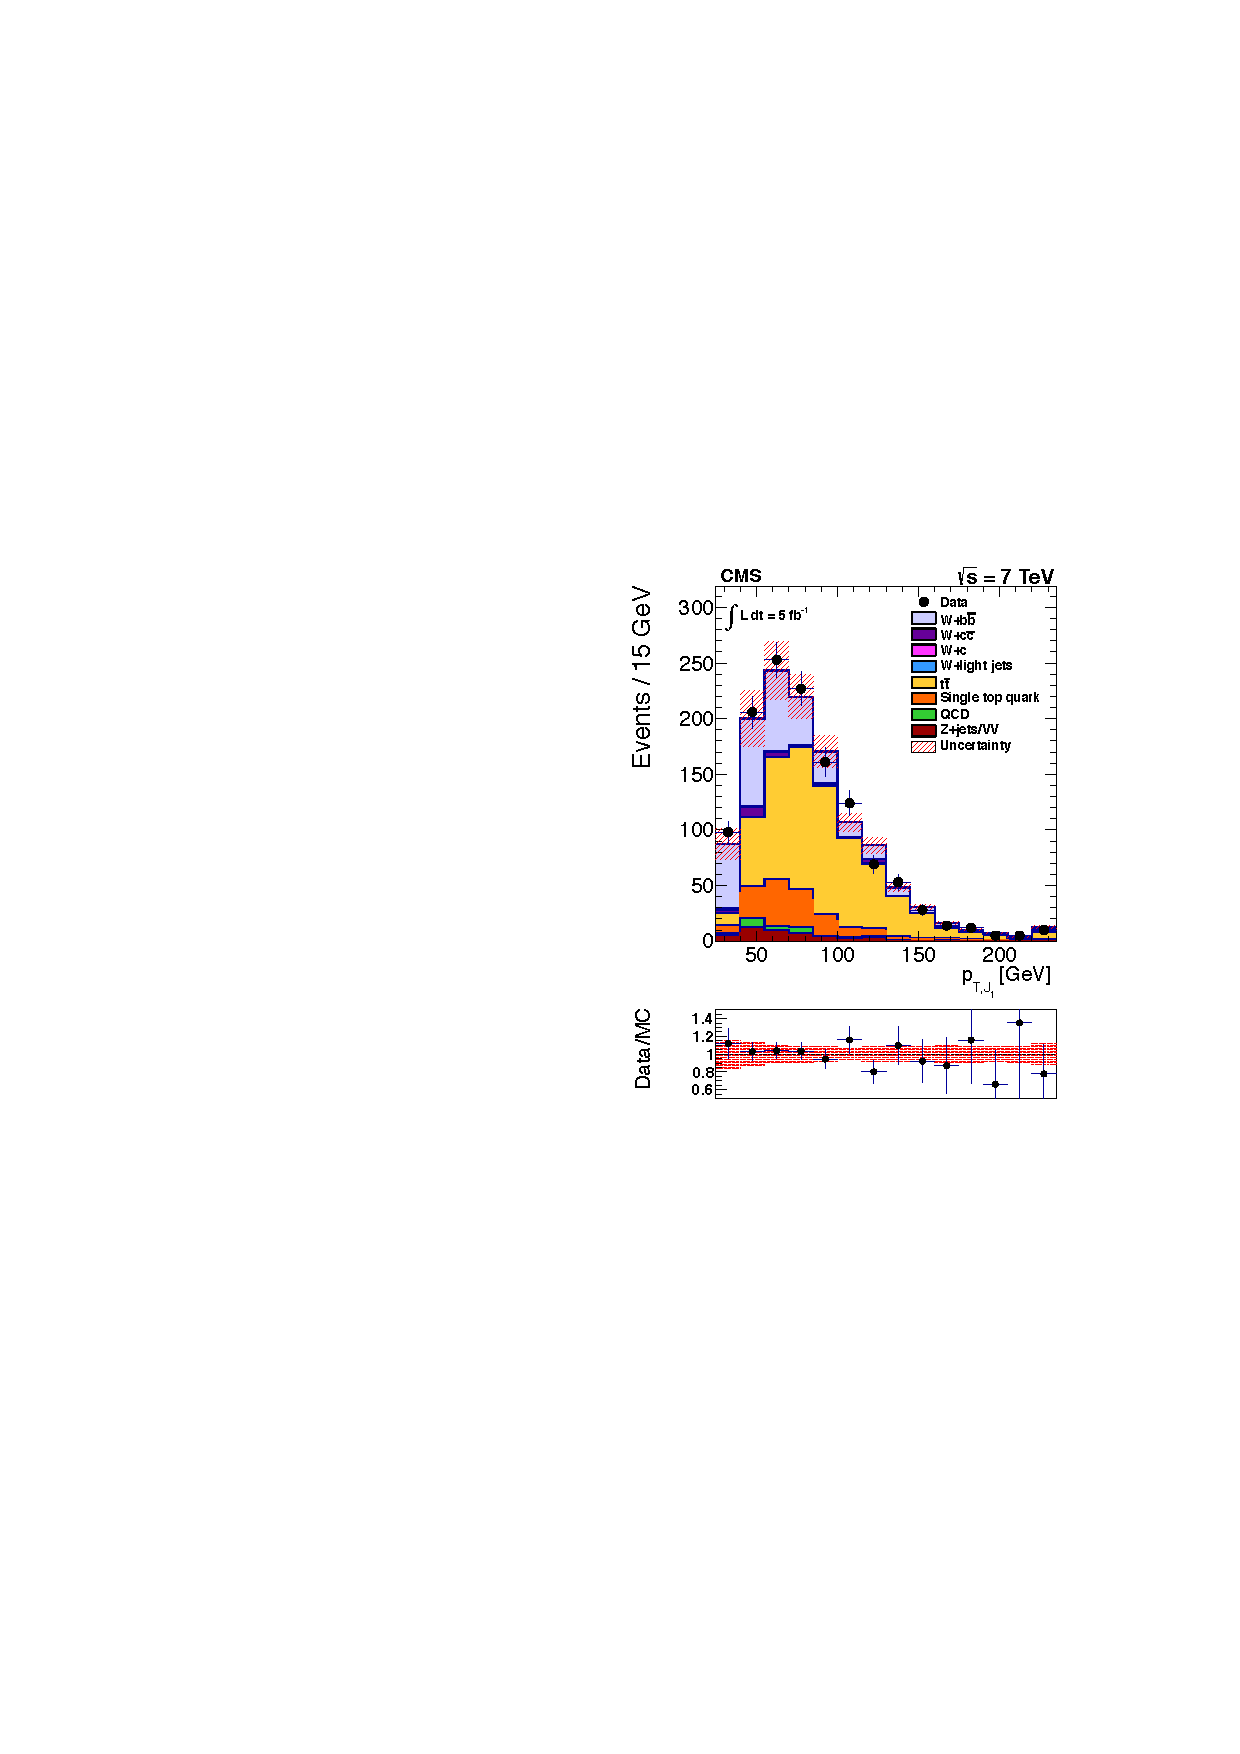
\includegraphics{Figures/cms_tot.pdf}
		%\rule{35em}{0.5pt}
	\caption[CMS Wbb total cross section measurement]{Leading jet transverse momentum distribution used for signal extraction in W+bb  total cross section measurement with the CMS experiment. \cite{Chatrchyan:2013uza} }
	\label{fig:cms_total}
\end{figure}